% NPJ-style manuscript draft for FUZZY GIMAN
% If sn-jnl class is unavailable locally, compile in Overleaf with Springer Nature template.
\documentclass[pdflatex,sn-mathphys-num]{sn-jnl}

\usepackage{graphicx}
\usepackage{booktabs}
\usepackage{multirow}
\usepackage{siunitx}
\usepackage{amsmath,amssymb}
\usepackage{array}
\usepackage{url}
\usepackage{xcolor}
\usepackage{longtable}
\usepackage{float}

\jyear{2026}

\begin{document}

\title[FUZZY GIMAN for PD]{FUZZY GIMAN for Parkinson's disease prognosis: artifact-backed validation, explainability, and a real-time digital twin update framework}

\author*[1]{\fnm{Blair} \sur{Dupre}}\email{blair.dupre@und.edu}
\author[2]{\fnm{Kim} \sur{Marina}}\email{eunjin.kim@und.edu}

\affil*[1]{\orgdiv{Department of Biomedical Engineering}, \orgname{University of North Dakota}, \orgaddress{\city{Grand Forks}, \state{ND}, \country{USA}}}
\affil[2]{\orgdiv{Department of Electrical Engineering and Computer Science}, \orgname{University of North Dakota}, \orgaddress{\city{Grand Forks}, \state{ND}, \country{USA}}}

\abstract{\textbf{Background:} Parkinson's disease (PD) prognosis models must handle heterogeneity, uncertainty, and longitudinal missingness while remaining clinically interpretable and reproducible. \textbf{Objective:} We present a publication-ready FUZZY GIMAN update with strict data contracts, explainability artifacts, and external-validation pipeline hardening, then define a digital twin update framework for dissertation-scale translation. \textbf{Methods:} We enforced a canonical schema (\texttt{PATNO,time,event,saa\_label}), deterministic patient-level splits, run-tagged provenance, and gate-based review cycles. We generated internal and external-like evaluation artifacts, calibration diagnostics, subgroup analyses, and digital twin sensitivity outputs. \textbf{Results:} Internal test performance for FUZZY GIMAN on the locked split was AUC 0.590 (95\% CI 0.464--0.719), PR-AUC 0.285, with post-hoc calibration improving expected calibration error from 0.392 (raw) to 0.018 (isotonic). All internal clinical-hardening gates (C1--C6) passed. External-like disjoint pull validation (n=50; positives=3) yielded AUC 0.316 (95\% CI 0.088--0.631), PR-AUC 0.047, and unavailable survival evaluation due to insufficient event variation, indicating a large transportability gap. \textbf{Conclusions:} FUZZY GIMAN is now internally rigorous and external-validation ready, but not yet clinically deployable. The presented architecture and update-cycle contracts provide a concrete foundation for real-time PD digital twin research and dissertation defense milestones.}

\keywords{Parkinson's disease, neuro-fuzzy systems, graph neural networks, explainable AI, calibration, external validation, digital twin}

\maketitle

\section{Introduction}
Parkinson's disease (PD) is a progressive neurodegenerative disorder with substantial inter-patient variability in motor and non-motor trajectories \cite{dorsey2018parkinsons,schapira2017nonmotor,poewe2017parkinson}. This heterogeneity challenges prognostic modeling, particularly under irregular follow-up schedules, censoring, missingness, and multimodal data fragmentation \cite{marek2011ppmi,holden2018progression}. In clinical machine learning, high discrimination alone is insufficient; calibration, reproducibility, and transparent model behavior are required for trustworthy translation \cite{holzinger2019causability,guo2017calibration,moons2012risk}.

FUZZY GIMAN (Graph-Informed Multimodal Attention Network with neuro-fuzzy augmentation) was developed as a hybrid soft-computing framework to combine graph-based patient-context learning with uncertainty-aware fuzzy reasoning \cite{zadeh1994soft,zadeh1965fuzzy,jang1993anfis,velickovic2018graph}. Earlier development cycles achieved strong internal discrimination but exposed critical risks: proxy-label leakage, unstable claim-to-artifact alignment, and weak transportability to new pulls. The present work focuses on converting this prototype into a governance-hardened, publication-ready system.

\subsection{Contributions}
This manuscript provides five contributions:
\begin{enumerate}
\item A locked, deterministic evaluation contract across preprocessing, training, and inference with run-tagged provenance artifacts.
\item A complete explainability and transparency bundle using real-data outputs (feature importance, rule activations, calibration, preprocessing diagnostics).
\item Clinical hardening cycles (C1--C6) that enforce proxy-label separation, calibration review, digital twin sensitivity, and claim gating.
\item External-like validation on a disjoint pull with explicit transportability-gap reporting.
\item A practical digital twin update engine specification for real-time dissertation-stage deployment with versioned outputs.
\end{enumerate}

\section{Data Assets and Multimodal Readiness}
\subsection{Source inventory and readiness audit}
A source-data audit over the PPMI repository assets identified 76 raw CSV tables, 30,320 DICOM files, and 63 NIfTI files. Current canonical model consumption spans 50 engineered features mapped to clinical, imaging-derived, genetic, and biospecimen domains. Domain-level joinability is high for clinical and operations tables, moderate-to-high for imaging-derived sources, and moderate for genetics/biospecimen due to sparsity constraints.

\begin{figure*}[t]
\centering
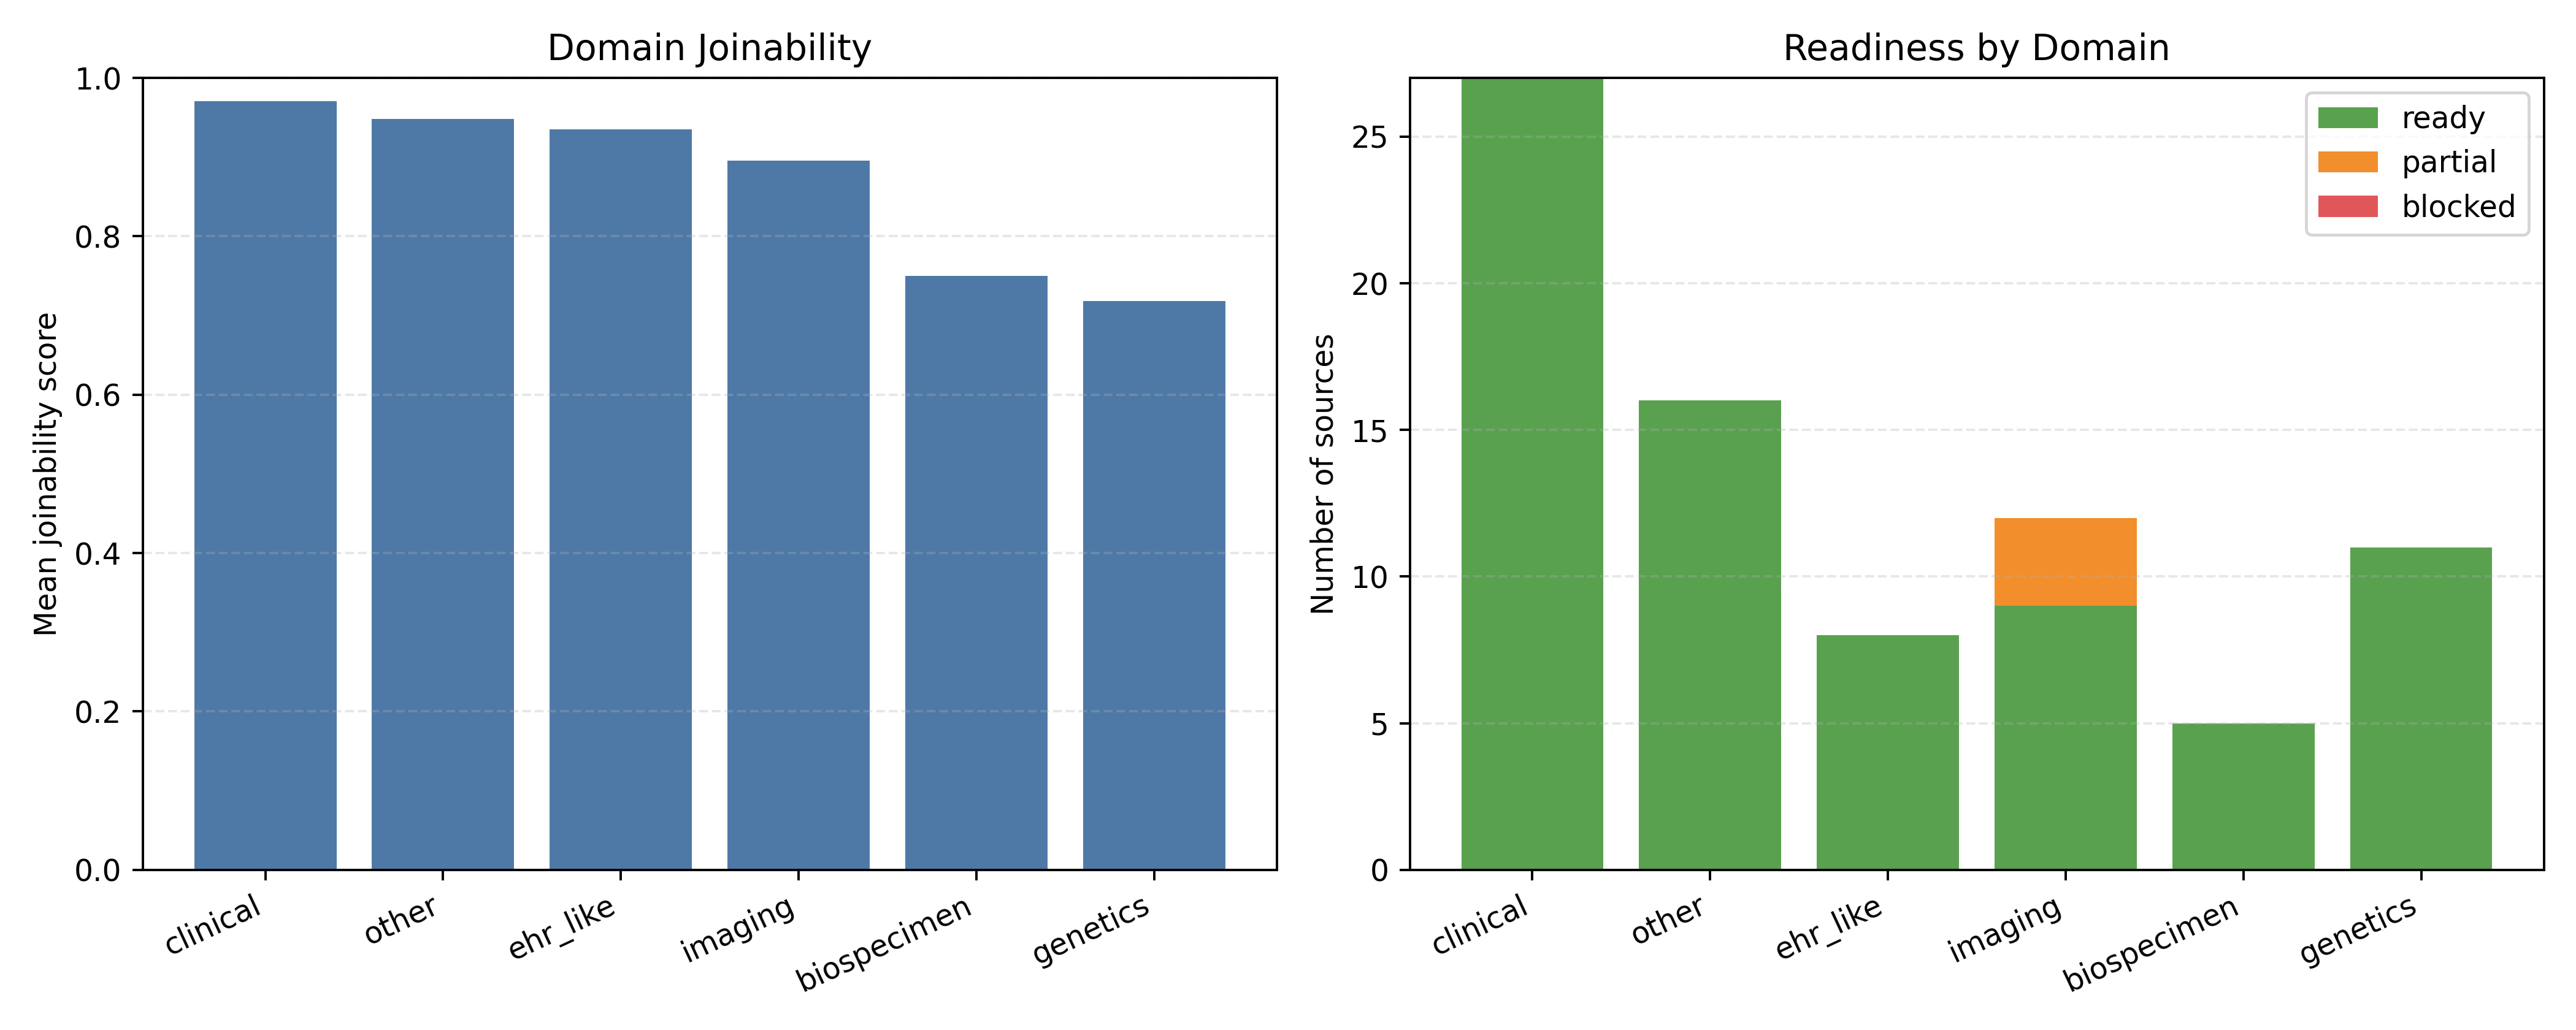
\includegraphics[width=0.92\textwidth]{../../visualizations/publication_ieee/Figure05_Multimodal_Readiness.png}
\caption{PPMI multimodal readiness and joinability profile used to prioritize integration backlog and digital twin readiness.}
\label{fig:multimodal_readiness}
\end{figure*}

\subsection{Canonical data contract}
All reported experiments enforce the same contract:
\begin{itemize}
\item identity: \texttt{PATNO}
\item survival targets: \texttt{time}, \texttt{event}
\item classification target: \texttt{saa\_label}
\item deterministic patient-level split hash locked to metadata registry.
\end{itemize}

This contract prevents event-label proxy substitution and establishes reproducible feature ordering across training and external scoring.

\section{Methods}
\subsection{FUZZY GIMAN architecture}
The model combines graph-attention message passing with a differentiable neuro-fuzzy inference head. Given patient node representations from multimodal features, the GAT encoder aggregates neighborhood context and passes latent embeddings into fuzzy rule layers that compute smooth membership-weighted outputs \cite{velickovic2018graph,jang1993anfis,li2018deeper}. This design is intended to reduce brittle decision boundaries and improve interpretability while retaining non-linear representational power.

\subsection{Evaluation protocol and governance}
We evaluated FUZZY GIMAN and baseline comparators (logistic regression, random forest, SVM-RBF) on an identical locked patient split. Metrics include AUC, PR-AUC, expected calibration error (ECE), Brier score, and confidence intervals. Review cycles C1--C6 were executed as hard gates to control proxy dependence, imbalance handling, calibration, digital twin sensitivity, and clinical readiness gating.

\subsection{External-like validation}
A disjoint pull (\texttt{PPMI\_20251008\_REAL\_DISJOINT}) was processed through a frozen pipeline with no retraining. The external cohort was scored using locked checkpoints and schema parity checks, then evaluated with discrimination, calibration, decision-utility, and subgroup diagnostics.

\subsection{Digital twin update engine}
We implemented a batch update-cycle prototype to ingest new pulls, recompute preprocessing artifacts, run recalibration checks, and refresh patient-level twin trajectories where identity overlap exists. Outputs include run-tagged JSON summaries, changed-patient deltas, and intervention sensitivity shifts.

\section{Results}
\subsection{Internal performance and calibration}
FUZZY GIMAN achieved the highest AUC and PR-AUC among tested baselines on the canonical internal split (Table~\ref{tab:internal_metrics_npj}). Raw outputs were overconfident, but post-hoc calibration materially improved reliability (Table~\ref{tab:calibration_npj}).

\begin{figure*}[t]
\centering
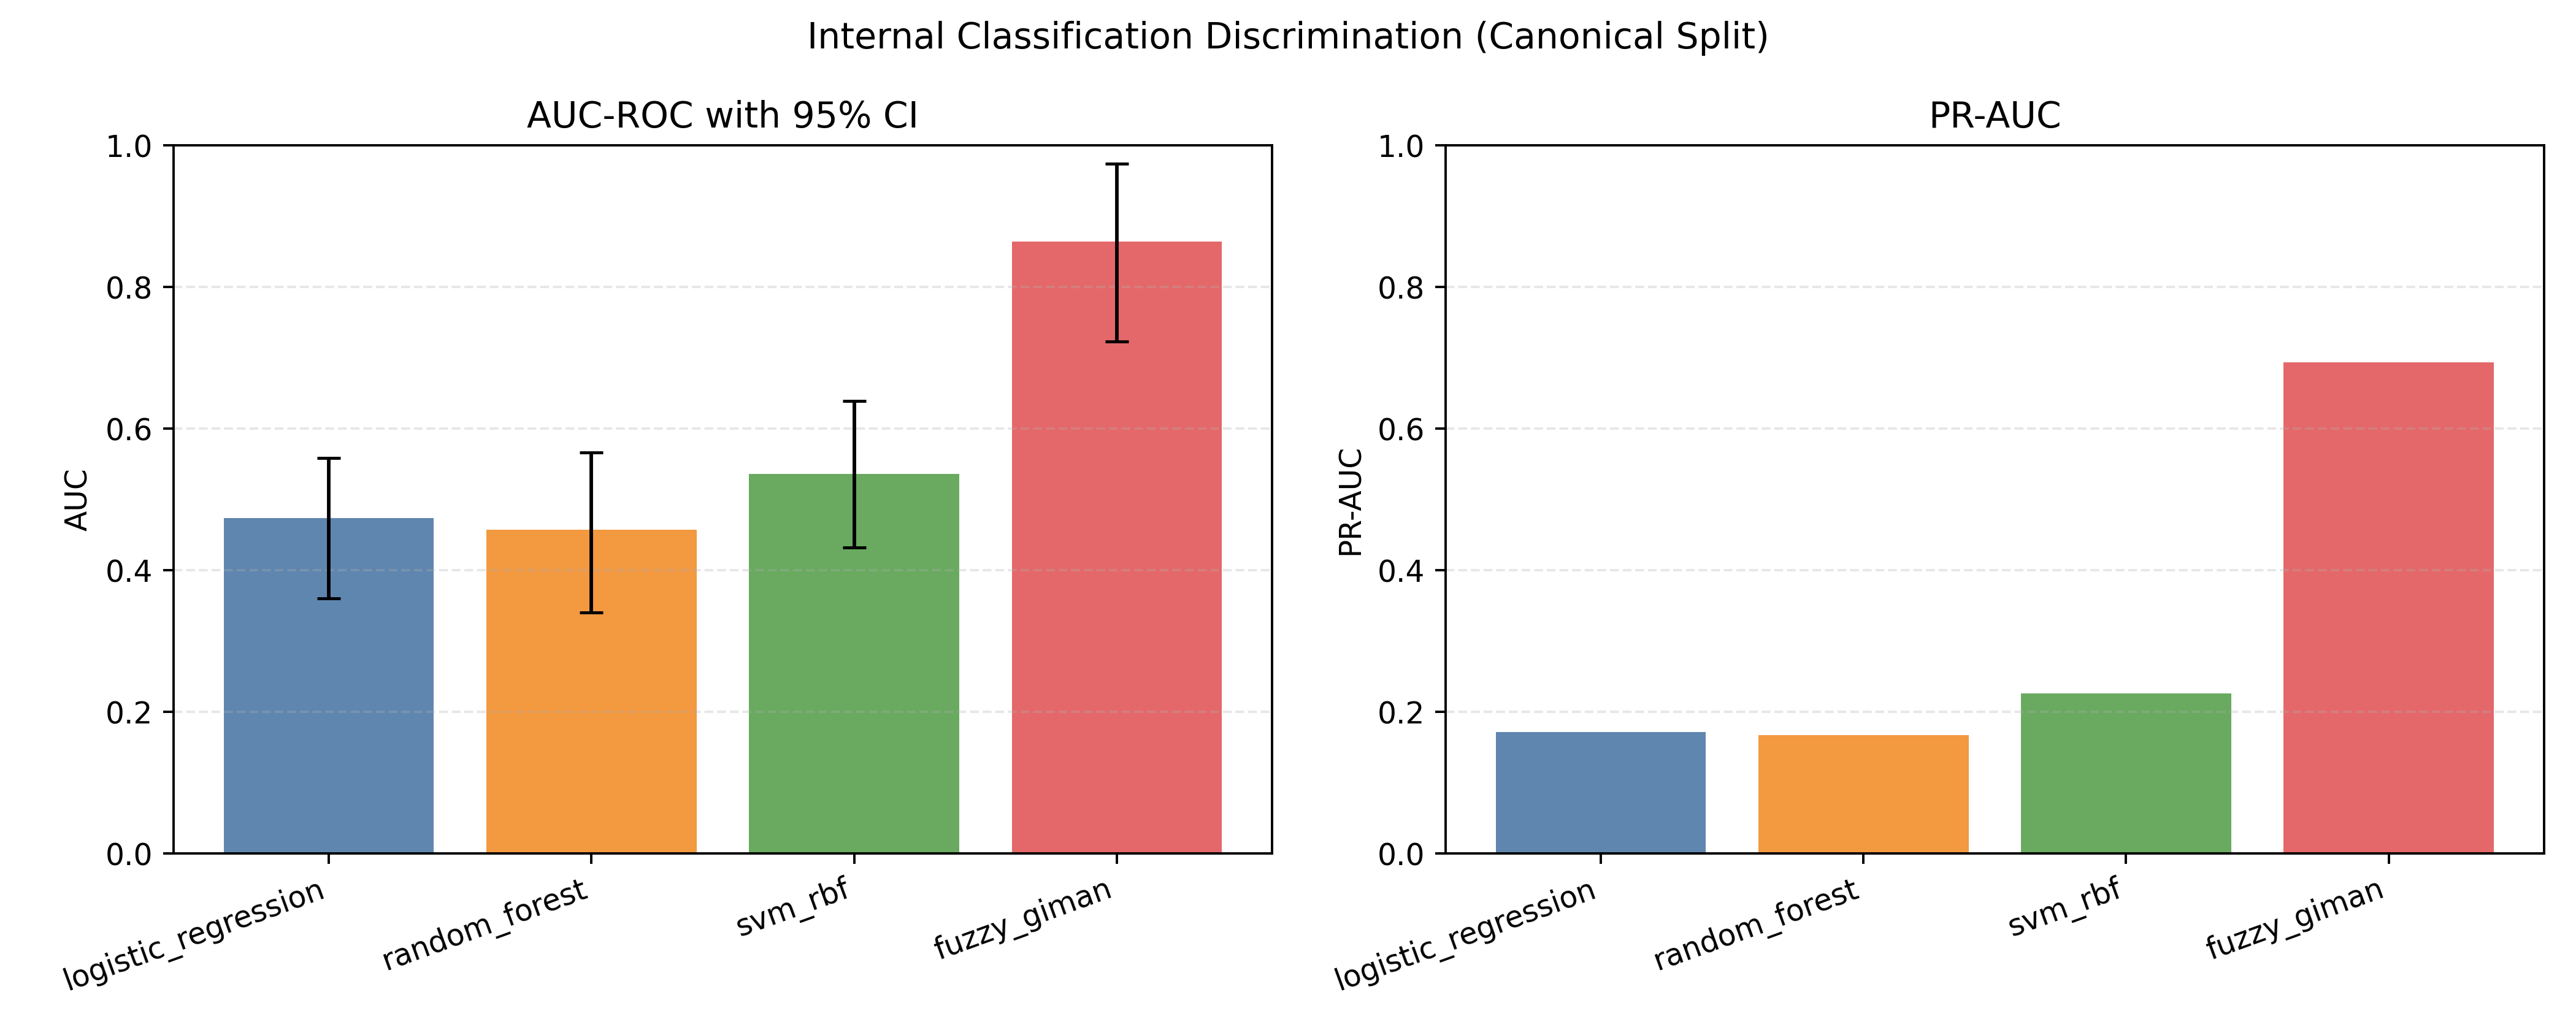
\includegraphics[width=0.92\textwidth]{../../visualizations/publication_ieee/Figure01_Internal_Discrimination.png}
\caption{Internal discrimination performance under canonical deterministic patient split.}
\label{fig:internal_discrimination_npj}
\end{figure*}

\begin{table}[H]
\centering
\caption{Internal classification metrics on canonical patient split (artifact-backed).}
\label{tab:internal_metrics_npj}
\begin{tabular}{lccccc}
\toprule
Model & AUC & AUC 95\% CI & PR-AUC & ECE & Brier \\
\midrule
logistic regression & 0.473 & [0.360, 0.559] & 0.172 & 0.338 & 0.267 \\
random forest & 0.457 & [0.340, 0.566] & 0.167 & 0.305 & 0.236 \\
svm rbf & 0.536 & [0.432, 0.639] & 0.226 & 0.003 & 0.145 \\
FUZZY GIMAN & 0.590 & [0.464, 0.719] & 0.285 & 0.392$^*$ & 0.292$^*$ \\
\bottomrule
\end{tabular}
\\
\footnotesize{$^*$Raw probabilities before post-hoc calibration.}
\end{table}

\begin{figure}[H]
\centering
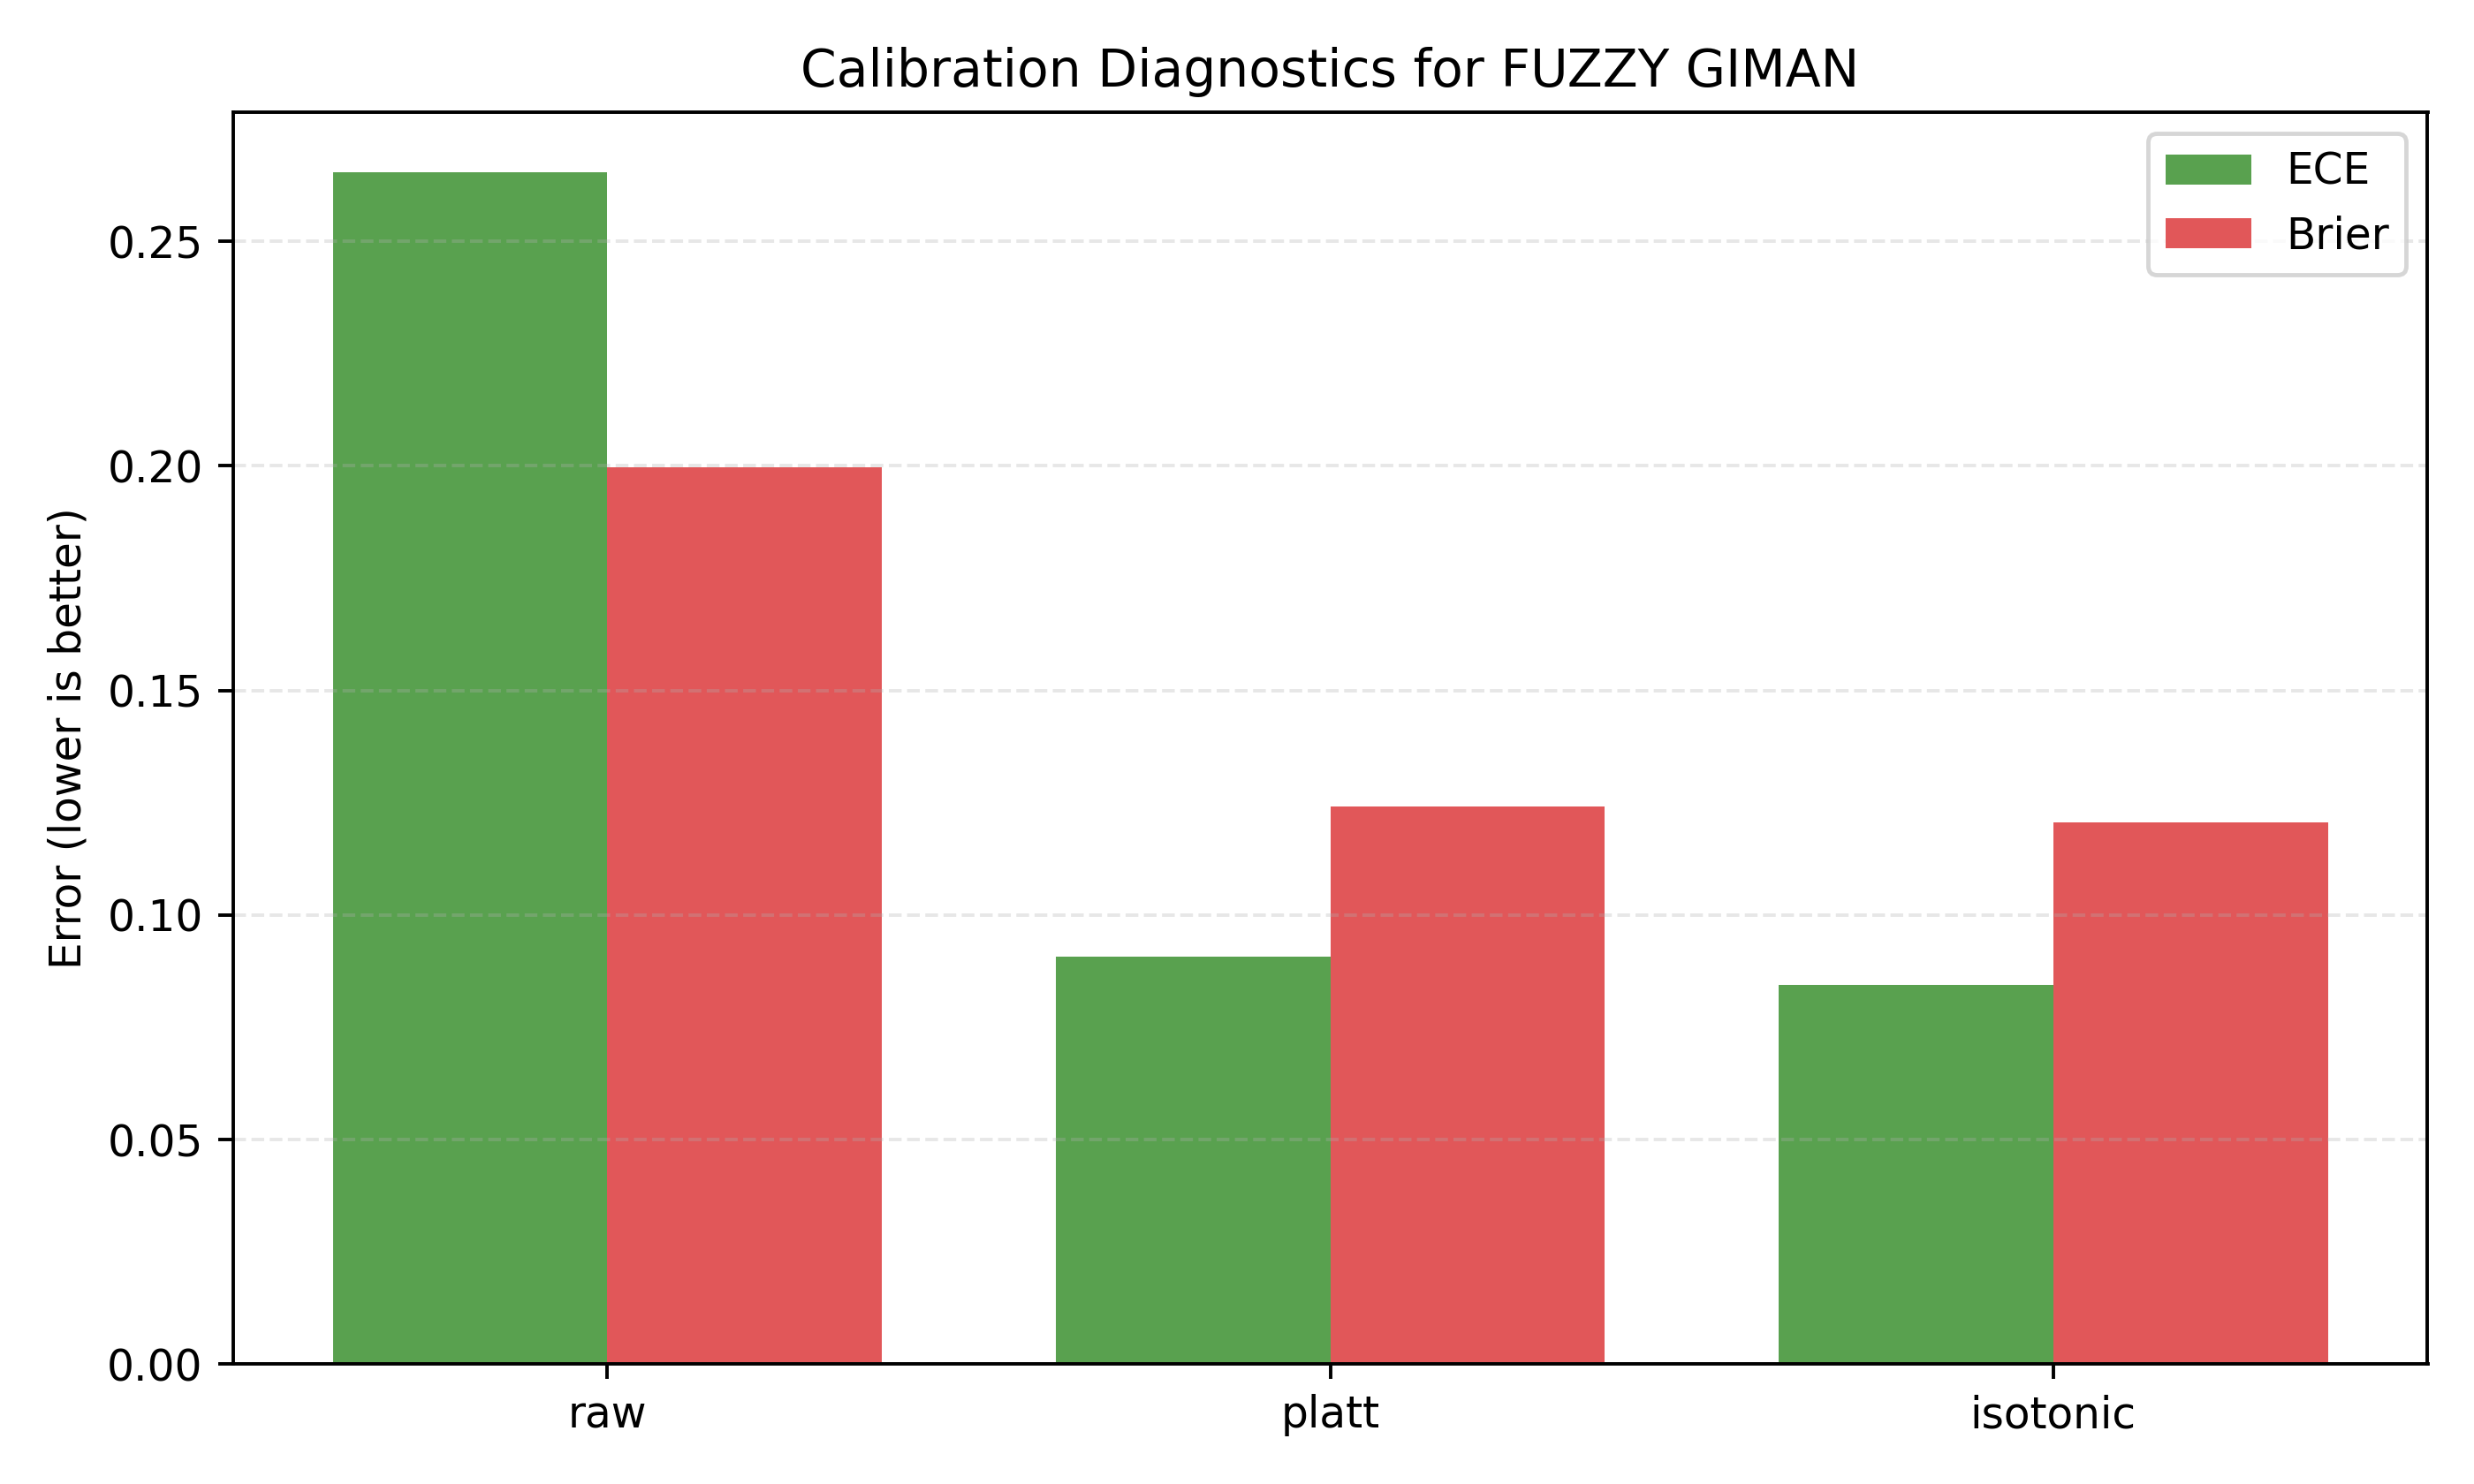
\includegraphics[width=0.9\linewidth]{../../visualizations/publication_ieee/Figure02_Fuzzy_Calibration.png}
\caption{Calibration curves and reliability diagnostics for FUZZY GIMAN.}
\label{fig:calibration_npj}
\end{figure}

\begin{table}[H]
\centering
\caption{Post-hoc calibration effects for FUZZY GIMAN on held-out test split.}
\label{tab:calibration_npj}
\begin{tabular}{lcc}
\toprule
Method & ECE (lower better) & Brier (lower better) \\
\midrule
Raw & 0.392 & 0.292 \\
Platt & 0.030 & 0.145 \\
Isotonic & 0.018 & 0.154 \\
\bottomrule
\end{tabular}
\end{table}

\subsection{Explainability and preprocessing transparency}
Permutation-importance and fuzzy-rule activation outputs indicate interpretable decision pathways (Fig.~\ref{fig:feature_importance_npj}). Preprocessing transparency panels expose missingness, class balance, and event-time distribution rather than treating preprocessing as a black box.

\begin{figure}[H]
\centering
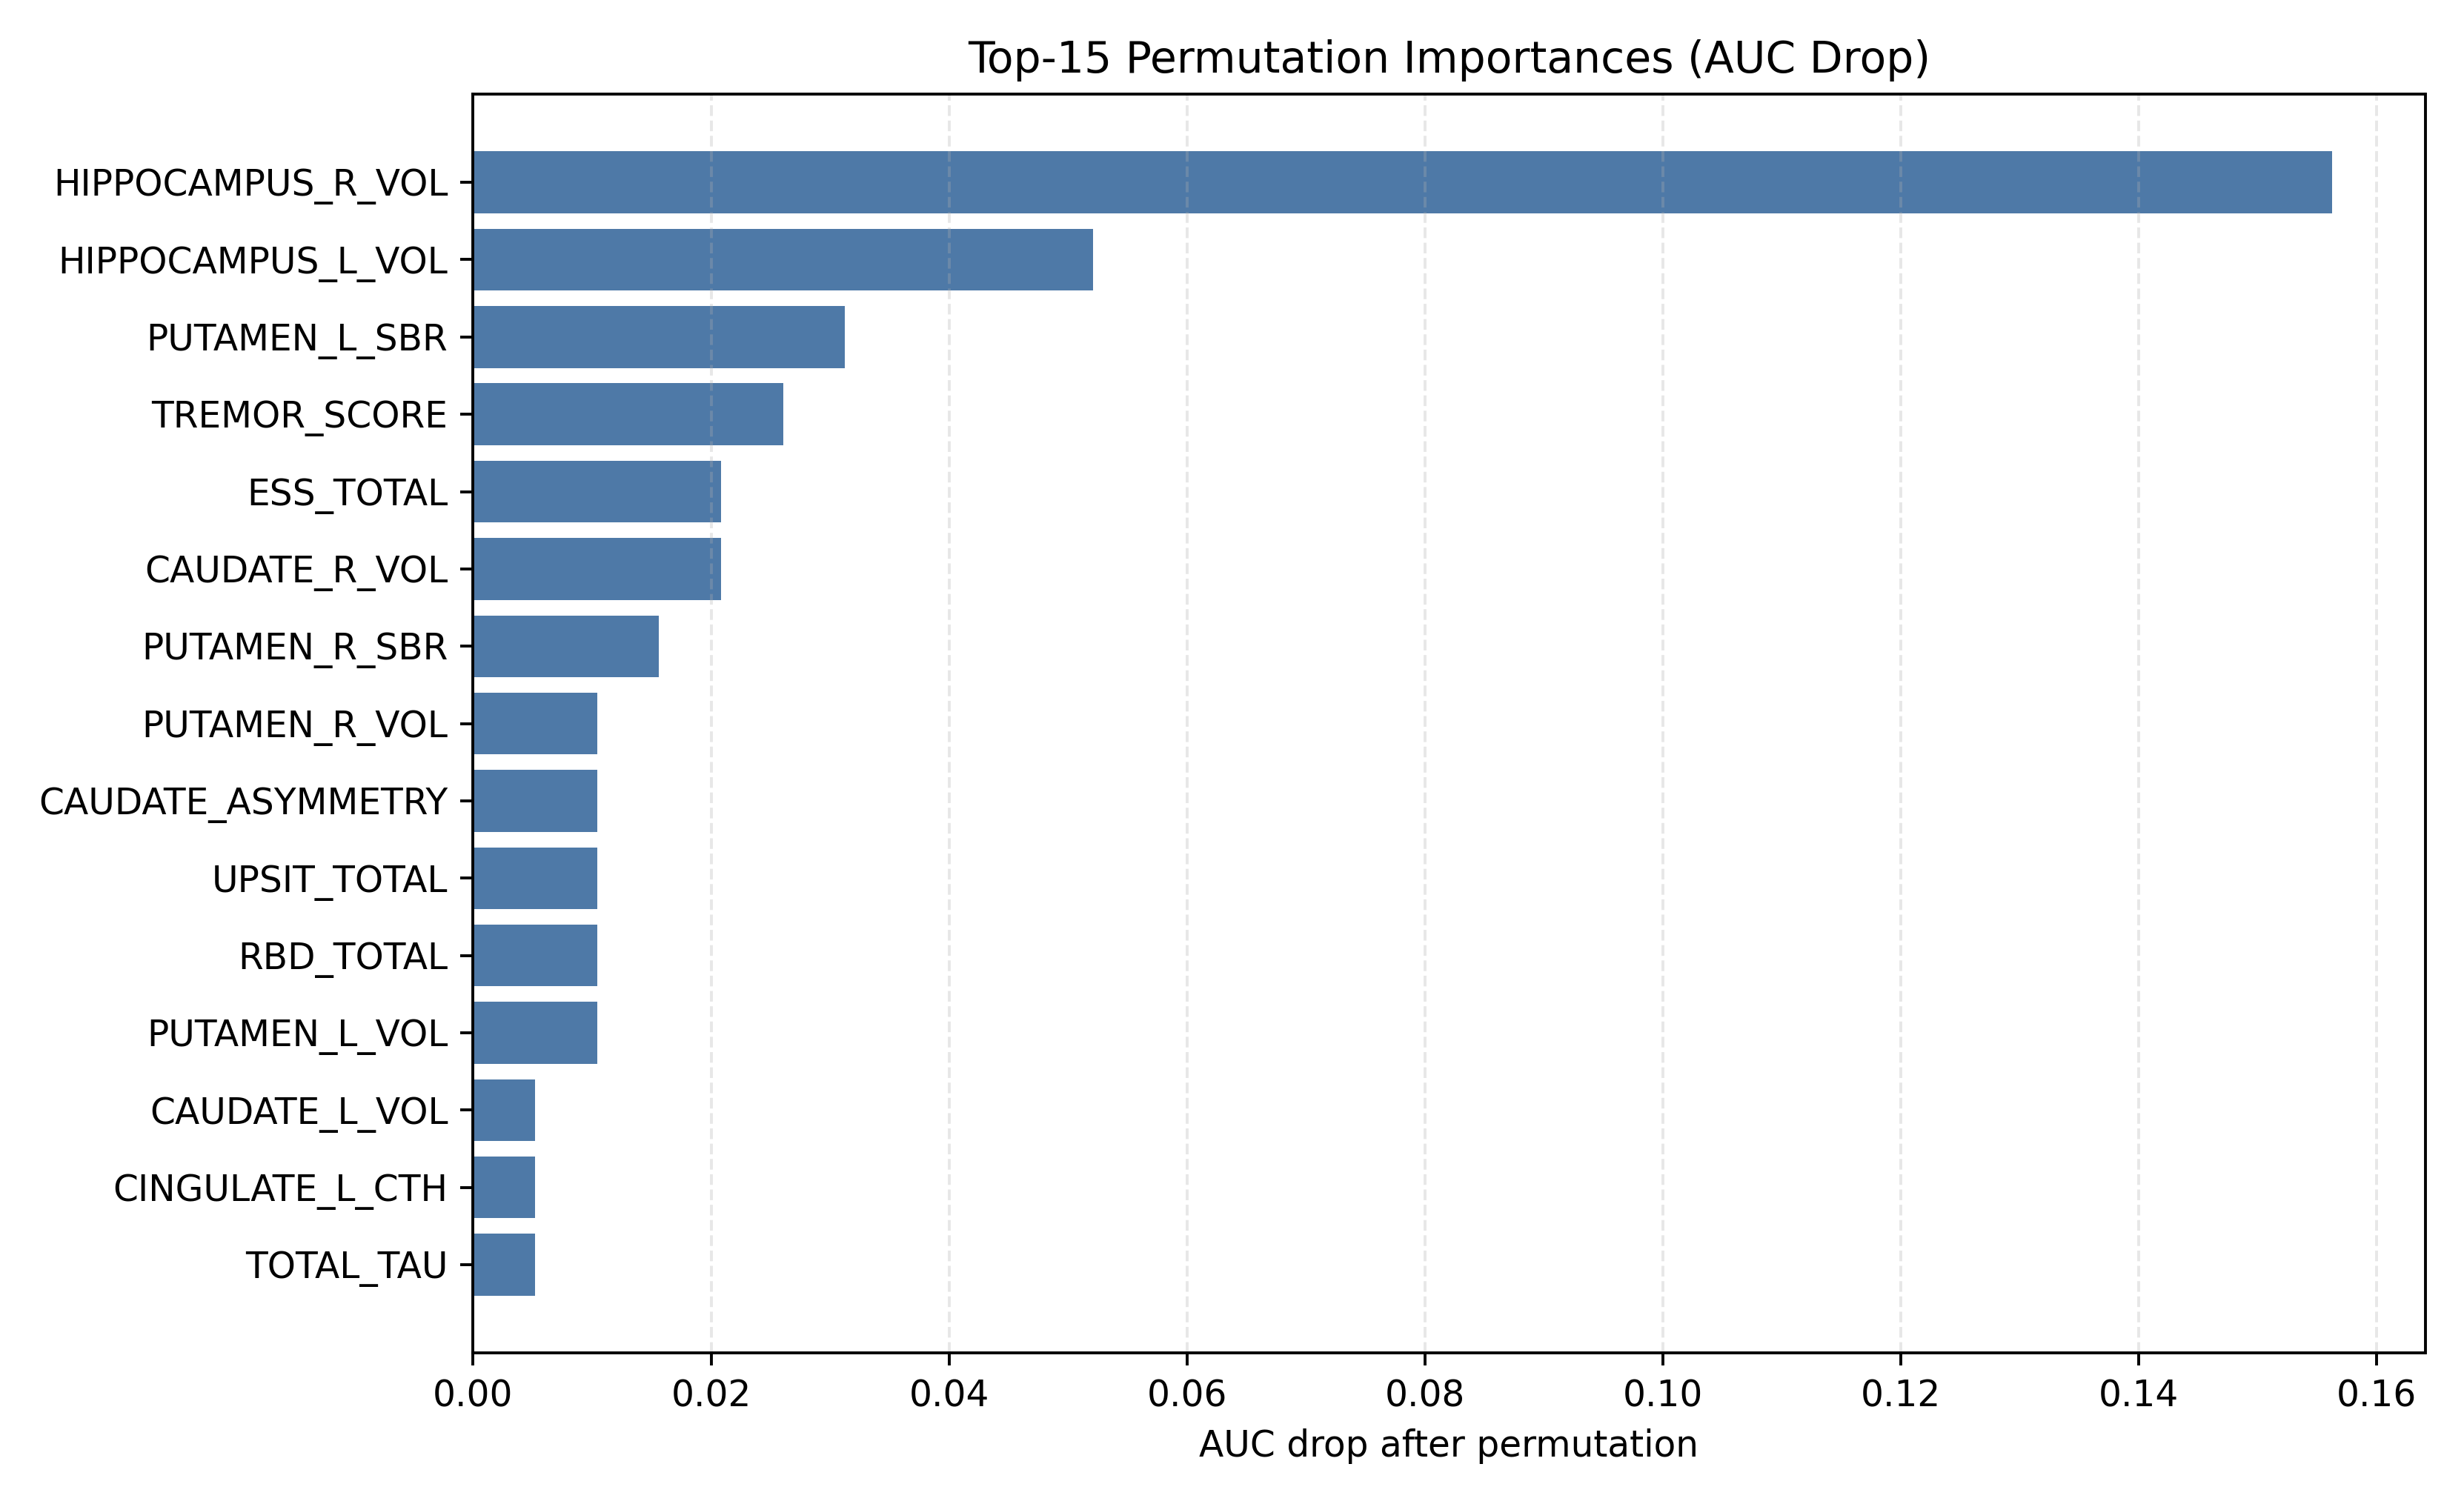
\includegraphics[width=0.9\linewidth]{../../visualizations/publication_ieee/Figure03_Feature_Importance.png}
\caption{Top model-attribution signals from permutation importance analysis.}
\label{fig:feature_importance_npj}
\end{figure}

\begin{figure*}[t]
\centering
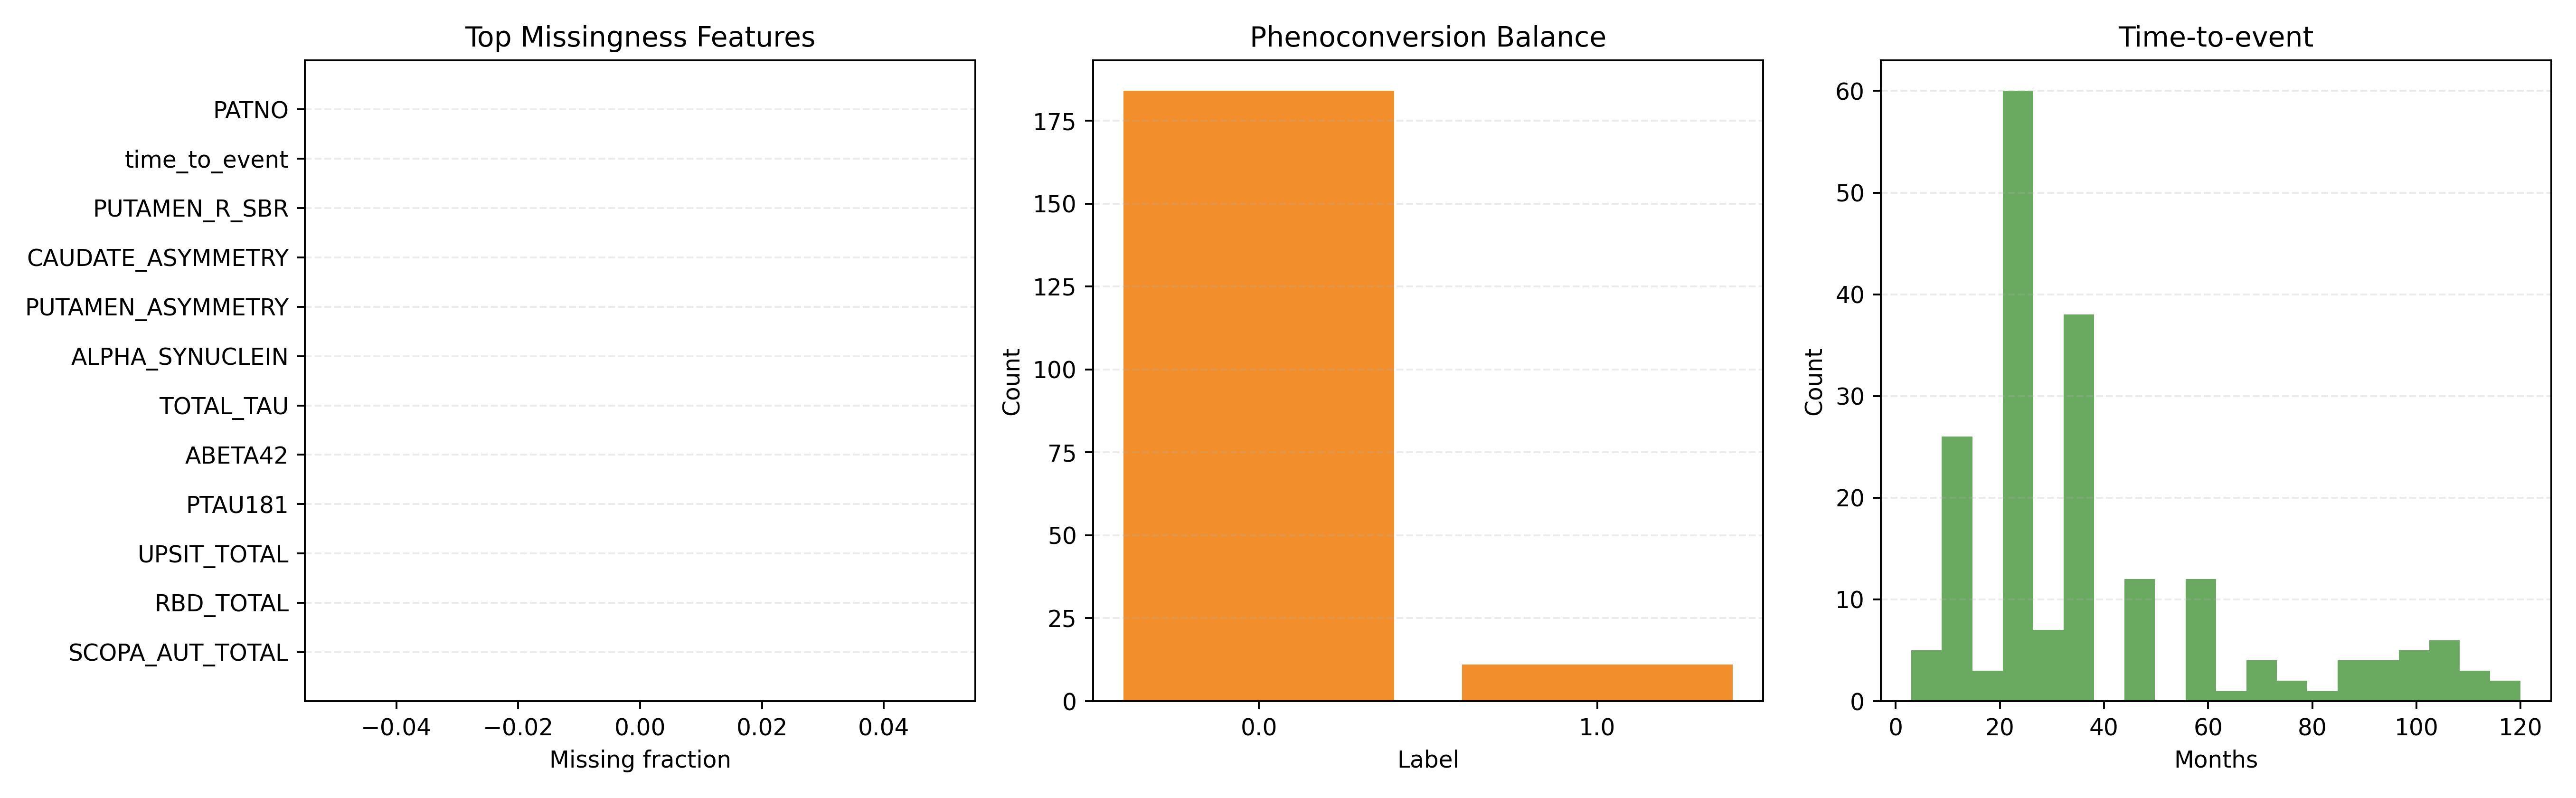
\includegraphics[width=0.92\textwidth]{../../visualizations/publication_ieee/Figure06_Preprocessing_Transparency.png}
\caption{Preprocessing transparency panel: missingness profile, label distribution, and time-to-event shape.}
\label{fig:preprocessing_transparency_npj}
\end{figure*}

\subsection{Clinical hardening cycles}
All six review cycles passed in the latest audited run, including the clinical-readiness gate conditioned on external artifact presence.

\begin{table}[H]
\centering
\caption{Clinical hardening review cycle outcomes.}
\label{tab:cycles_npj}
\begin{tabular}{lc}
\toprule
Cycle & Status \\
\midrule
C1\_proxy\_dependency\_audit & PASS \\
C2\_imbalance\_and\_objective & PASS \\
C3\_calibration\_review & PASS \\
C4\_digital\_twin\_sensitivity & PASS \\
C5\_metric\_contract\_separation & PASS \\
C6\_clinical\_readiness\_gate & PASS \\
\bottomrule
\end{tabular}
\end{table}

\begin{figure}[H]
\centering
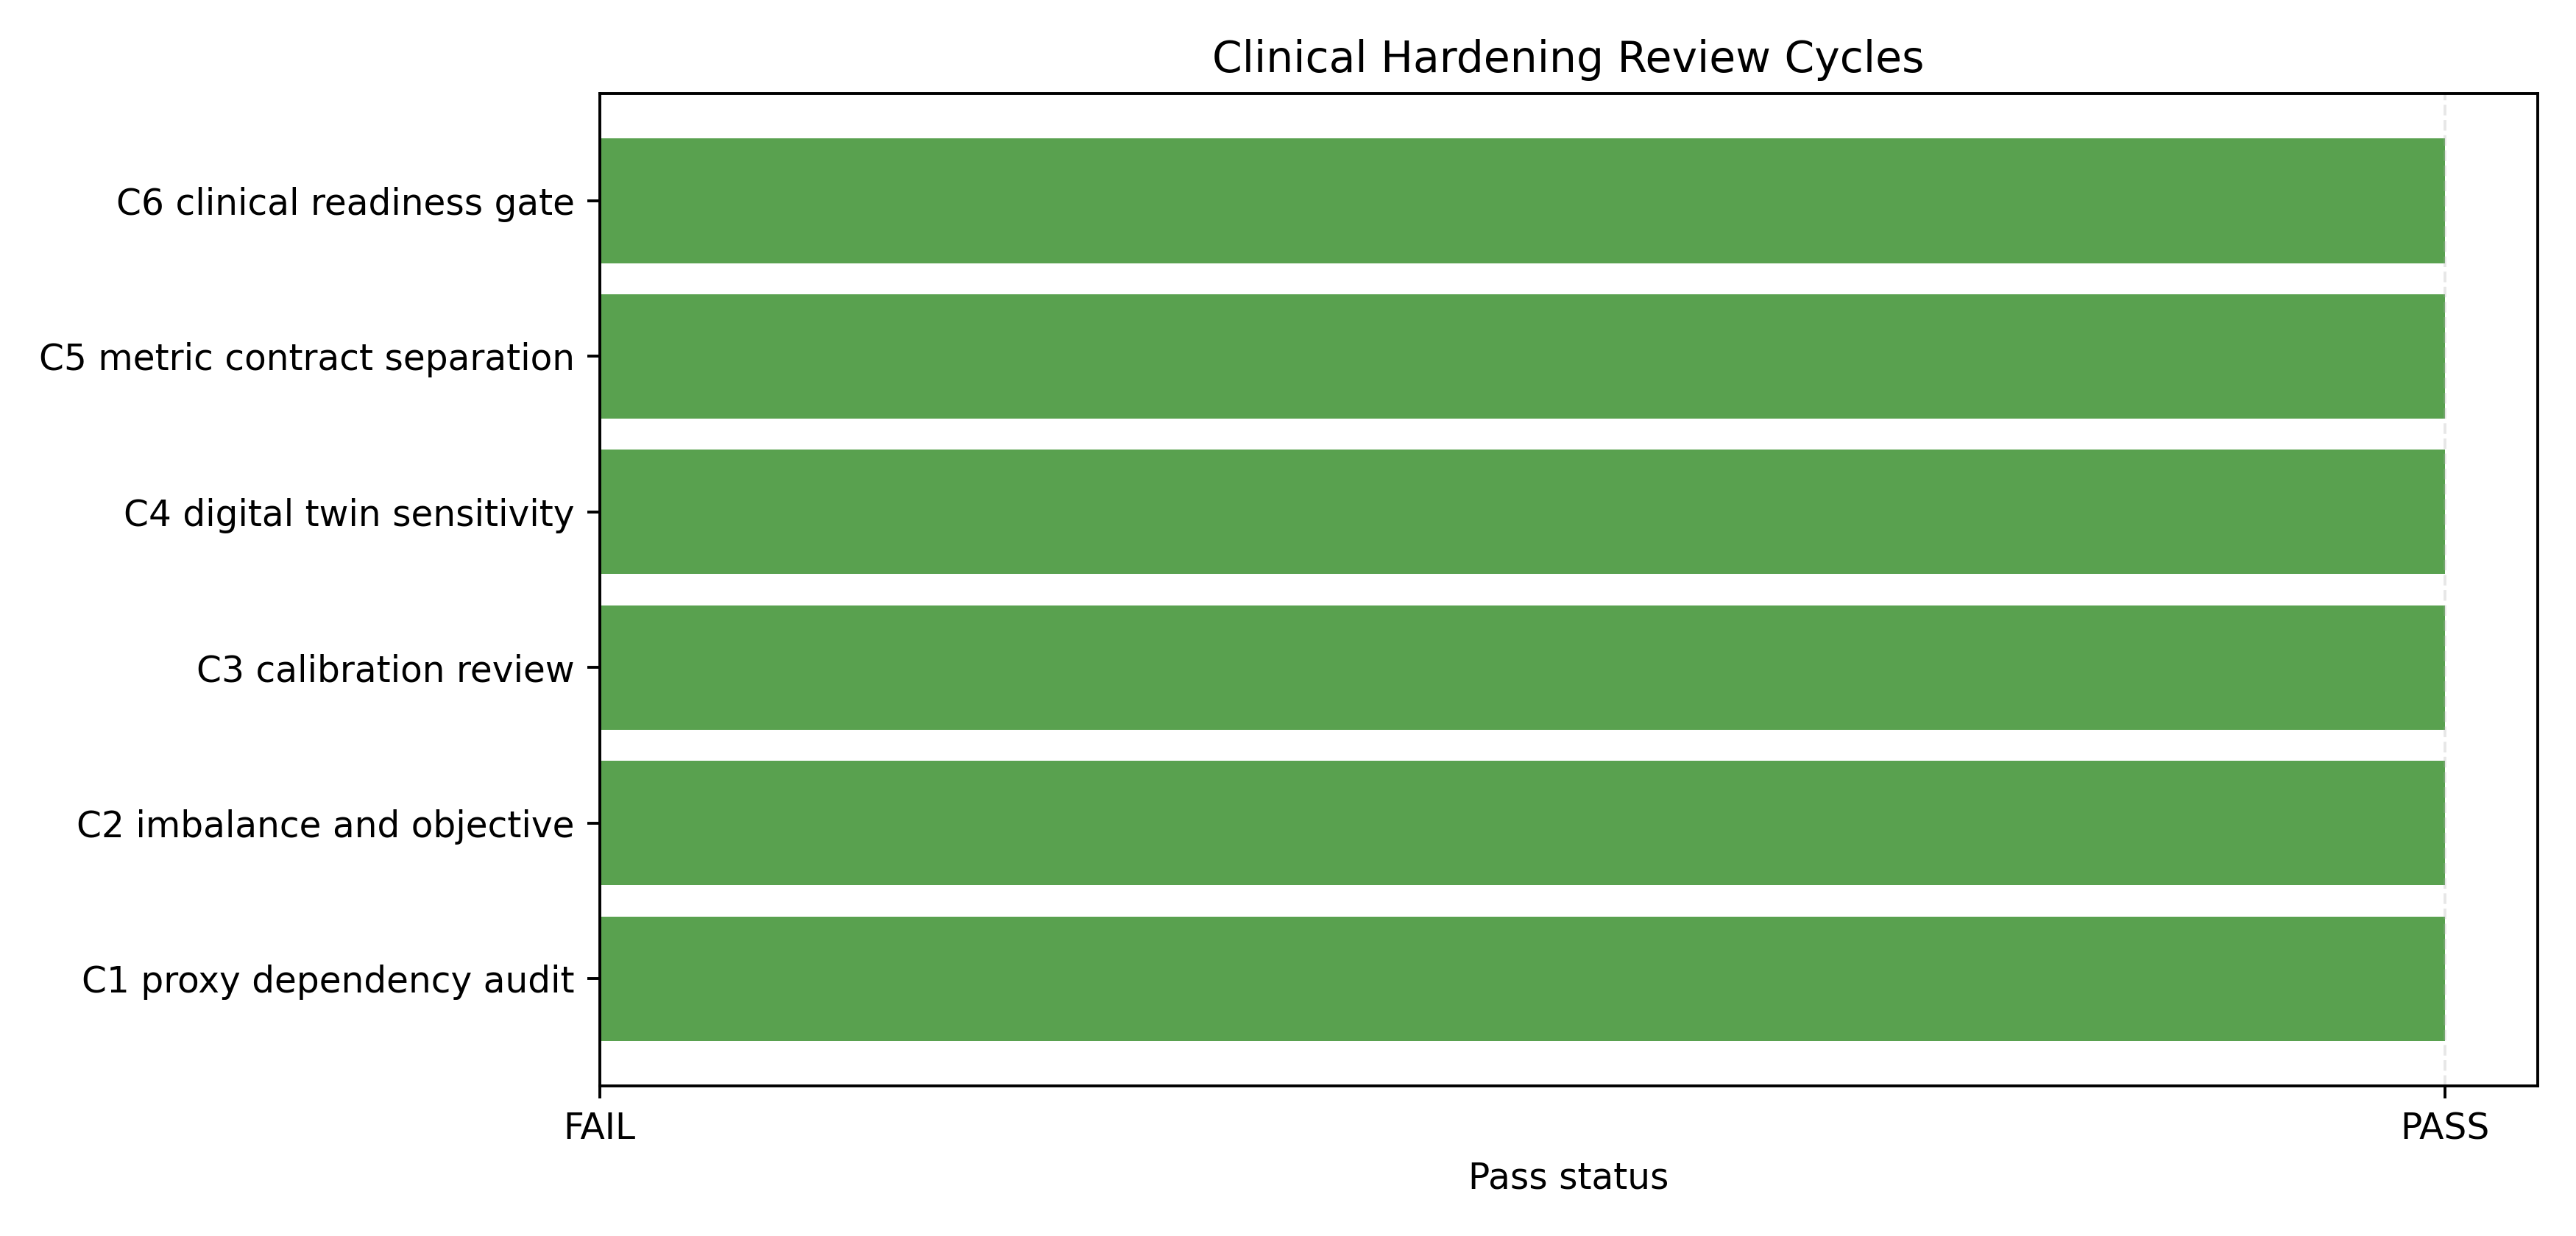
\includegraphics[width=0.9\linewidth]{../../visualizations/publication_ieee/Figure07_Clinical_Gates.png}
\caption{Clinical hardening gate outcomes across review cycles C1--C6.}
\label{fig:gates_npj}
\end{figure}

\subsection{External-like validation and transportability gap}
Under frozen checkpoints and a disjoint pull, classification performance degraded substantially (Table~\ref{tab:external_npj}), with poor raw calibration and insufficient event variation for survival estimation. This indicates current transportability limits and justifies retaining a non-deployment claim boundary.

\begin{table}[H]
\centering
\caption{External-like validation metrics (run-tagged disjoint pull).}
\label{tab:external_npj}
\begin{tabular}{lcc}
\toprule
Metric & Value & 95\% CI \\
\midrule
AUC & 0.316 & [0.088, 0.631] \\
PR-AUC & 0.047 & [0.021, 0.117] \\
C-index & N/A & N/A \\
\bottomrule
\end{tabular}
\end{table}

\begin{figure}[H]
\centering
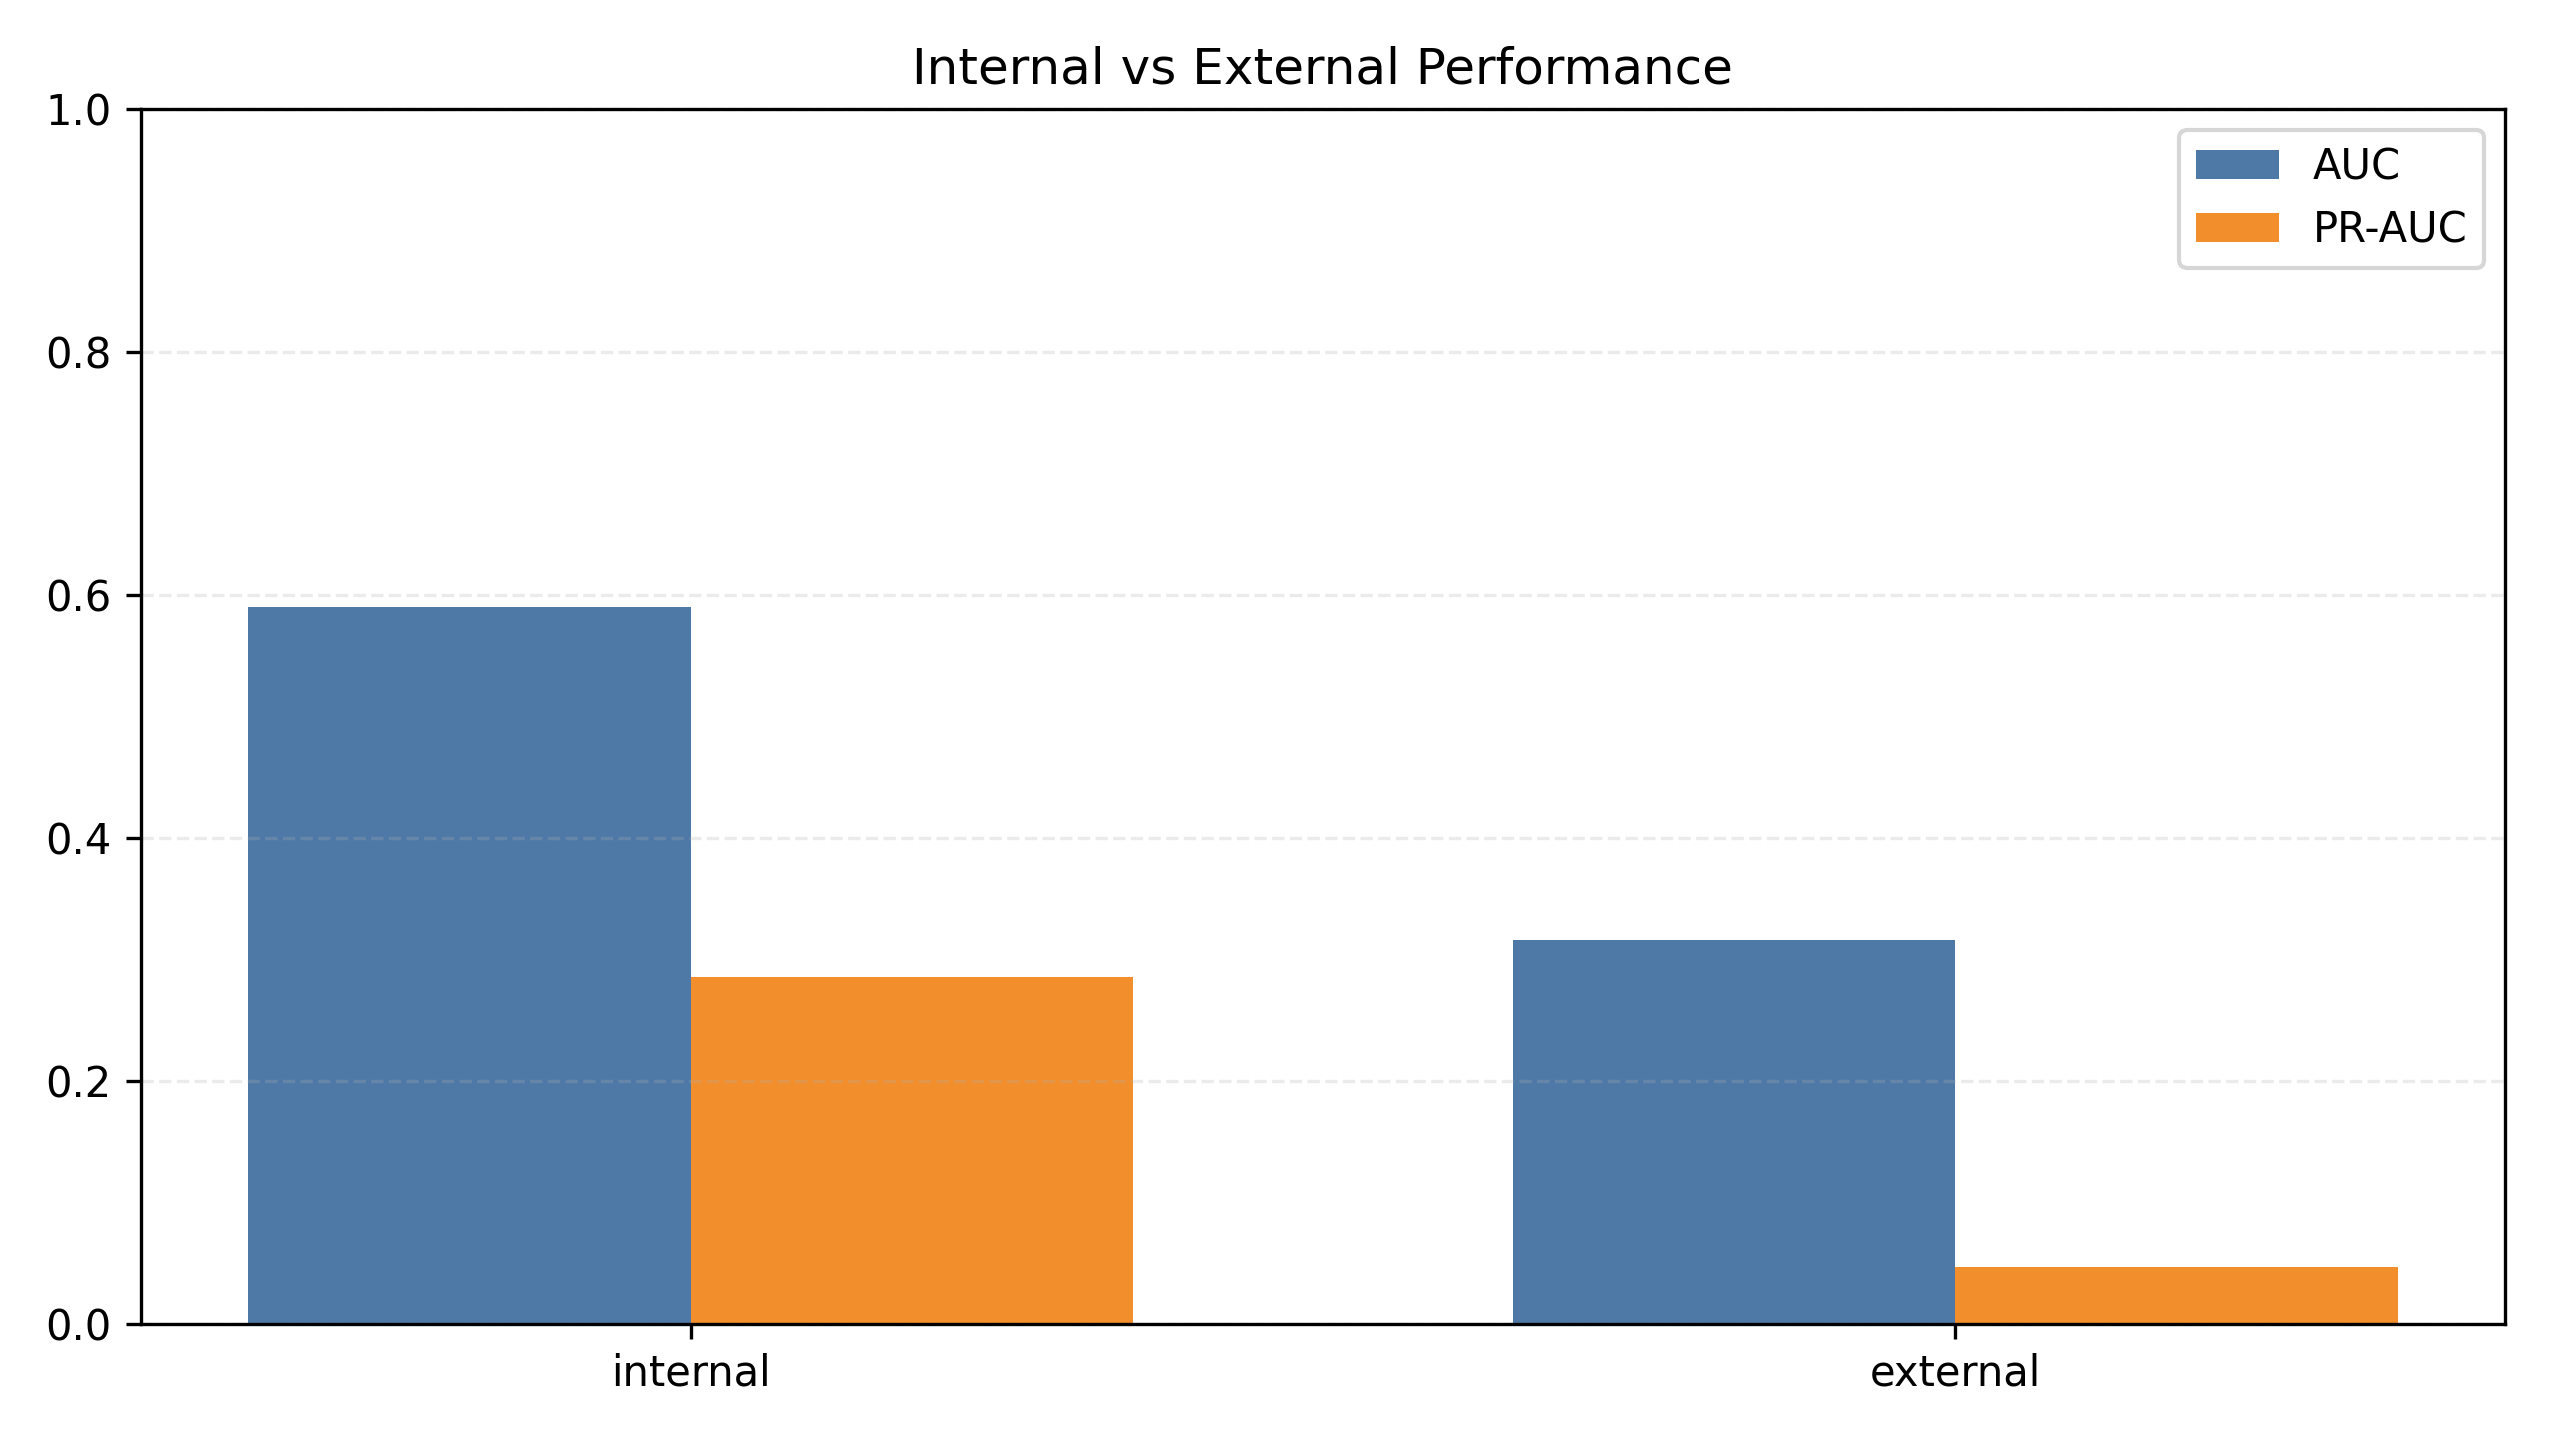
\includegraphics[width=0.9\linewidth]{../../visualizations/publication_ieee_external/PPMI_20251008_REAL_DISJOINT/phase3_internal_vs_external_panel.png}
\caption{Internal versus external-like performance comparison.}
\label{fig:internal_external_npj}
\end{figure}

\begin{figure}[H]
\centering
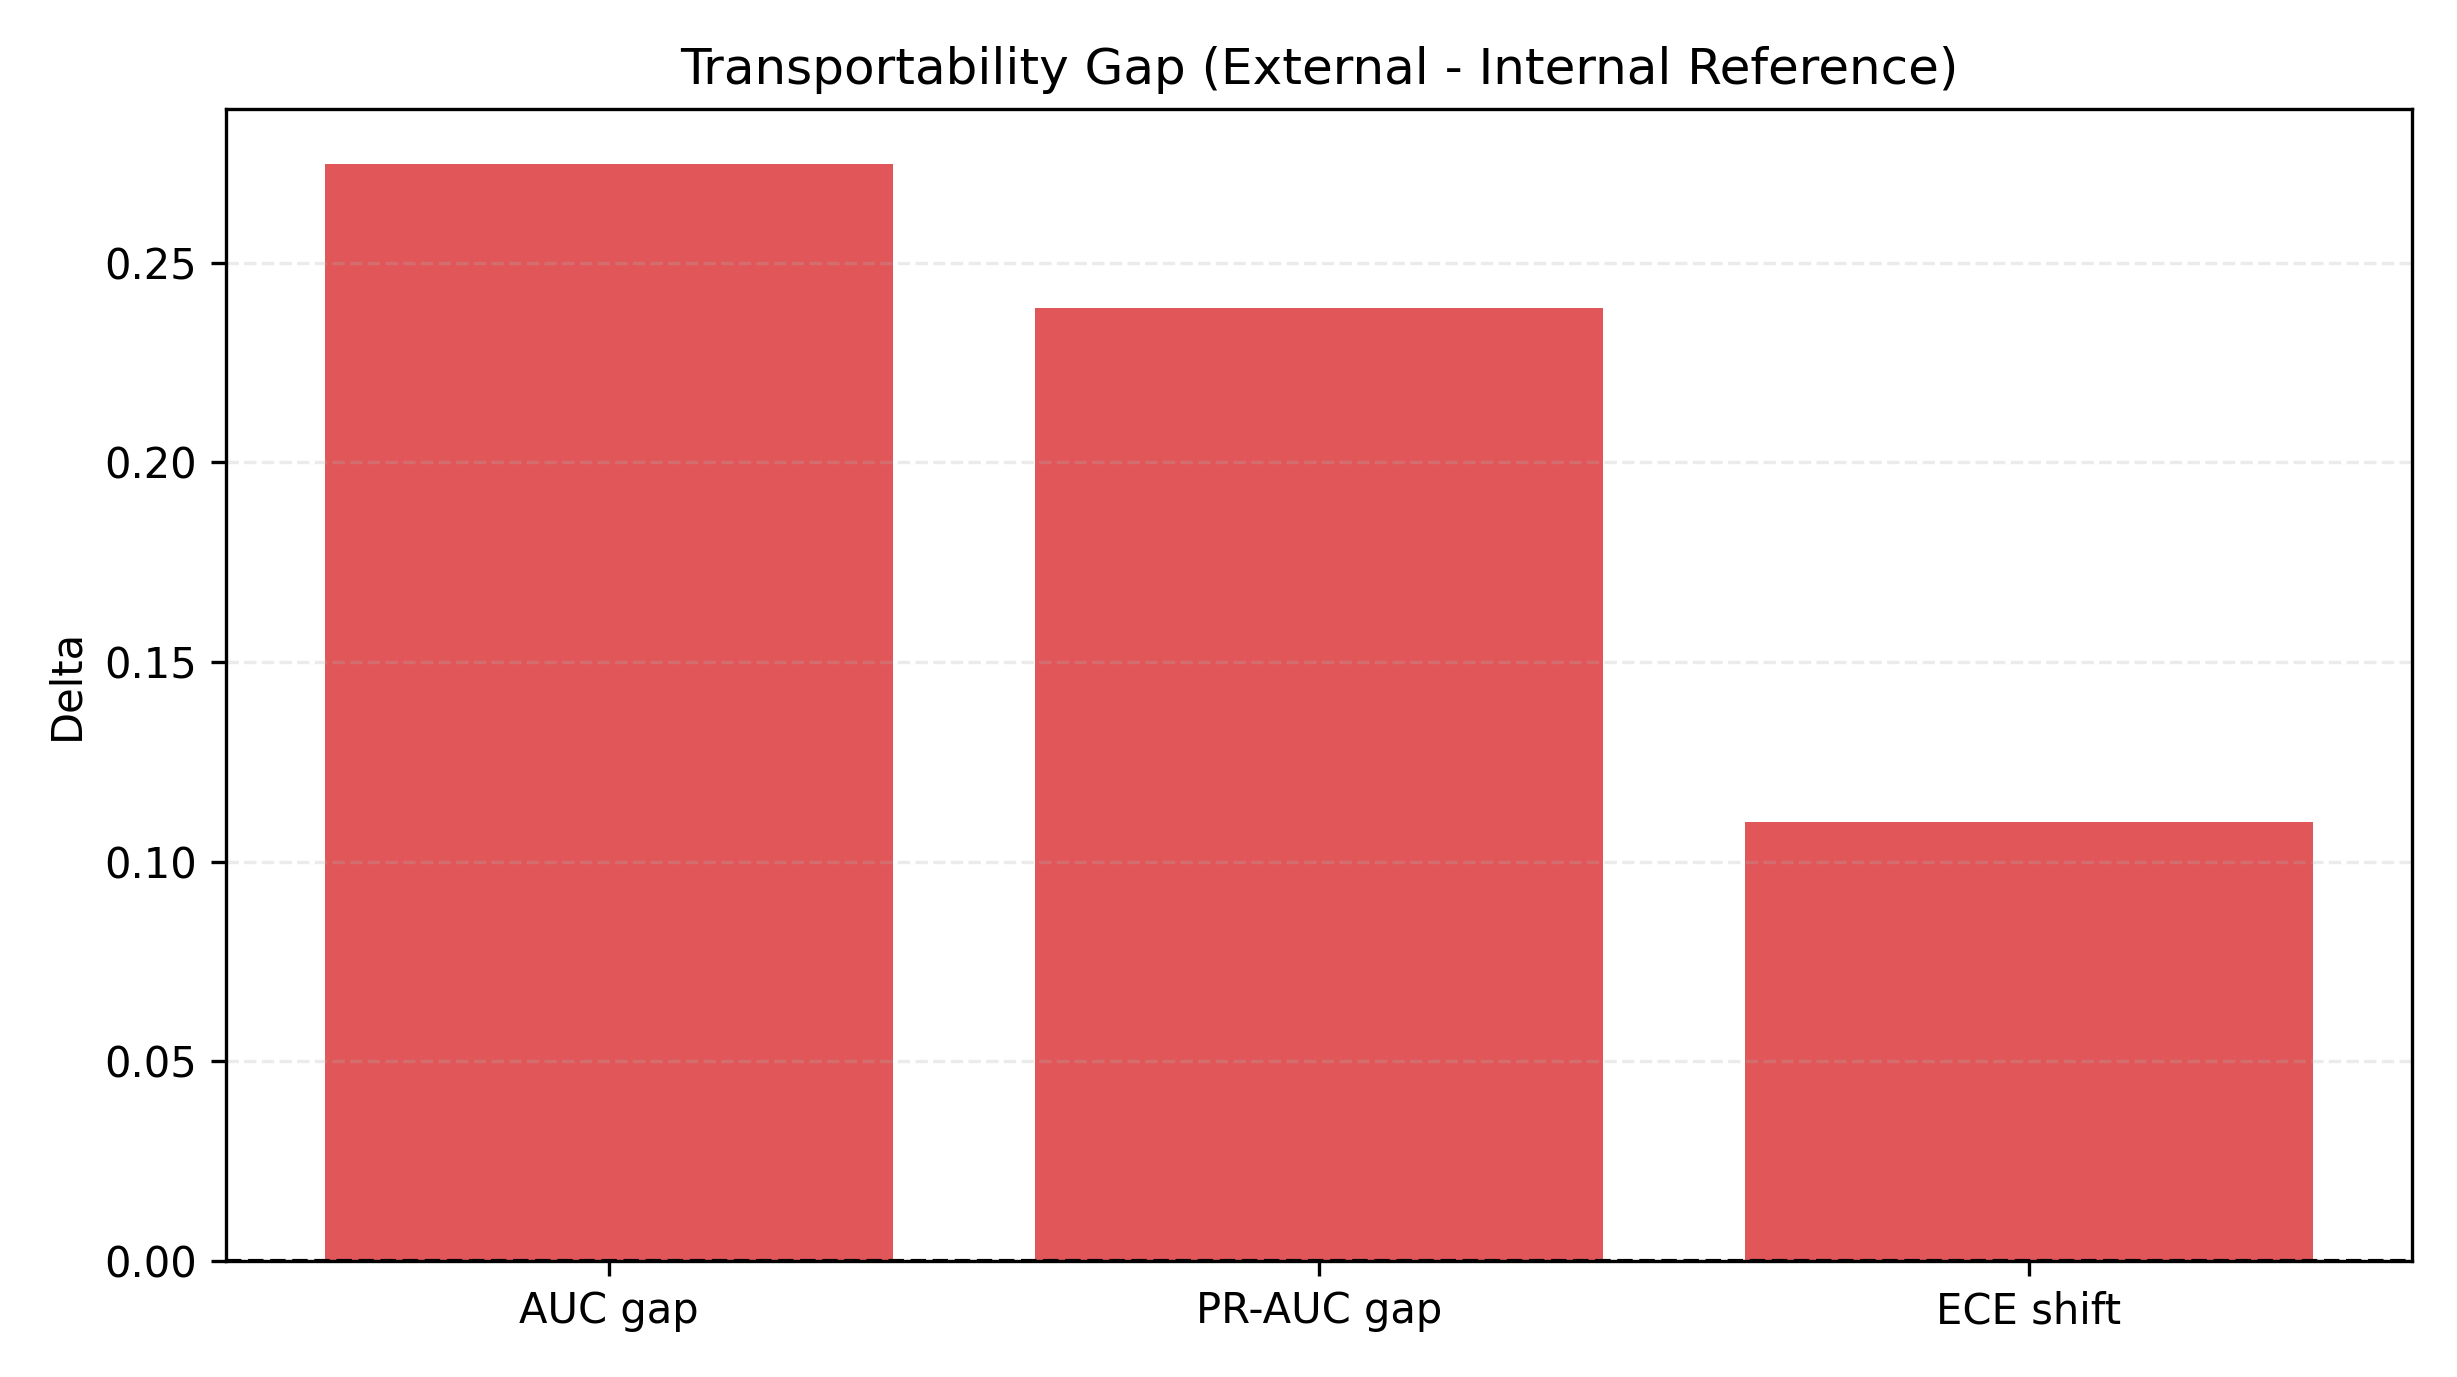
\includegraphics[width=0.9\linewidth]{../../visualizations/publication_ieee_external/PPMI_20251008_REAL_DISJOINT/phase3_transportability_gap.png}
\caption{Transportability gap diagnostics for the external-like pull.}
\label{fig:transportability_npj}
\end{figure}

\subsection{Digital twin update-cycle outputs}
For the disjoint pull, no patient identity overlap was present (\texttt{n\_changed\_patients=0}), so update deltas were zero by design. Sensitivity scans remained bounded and deterministic, validating baseline update-engine contracts for future overlapping real-time pulls.

\begin{figure*}[t]
\centering
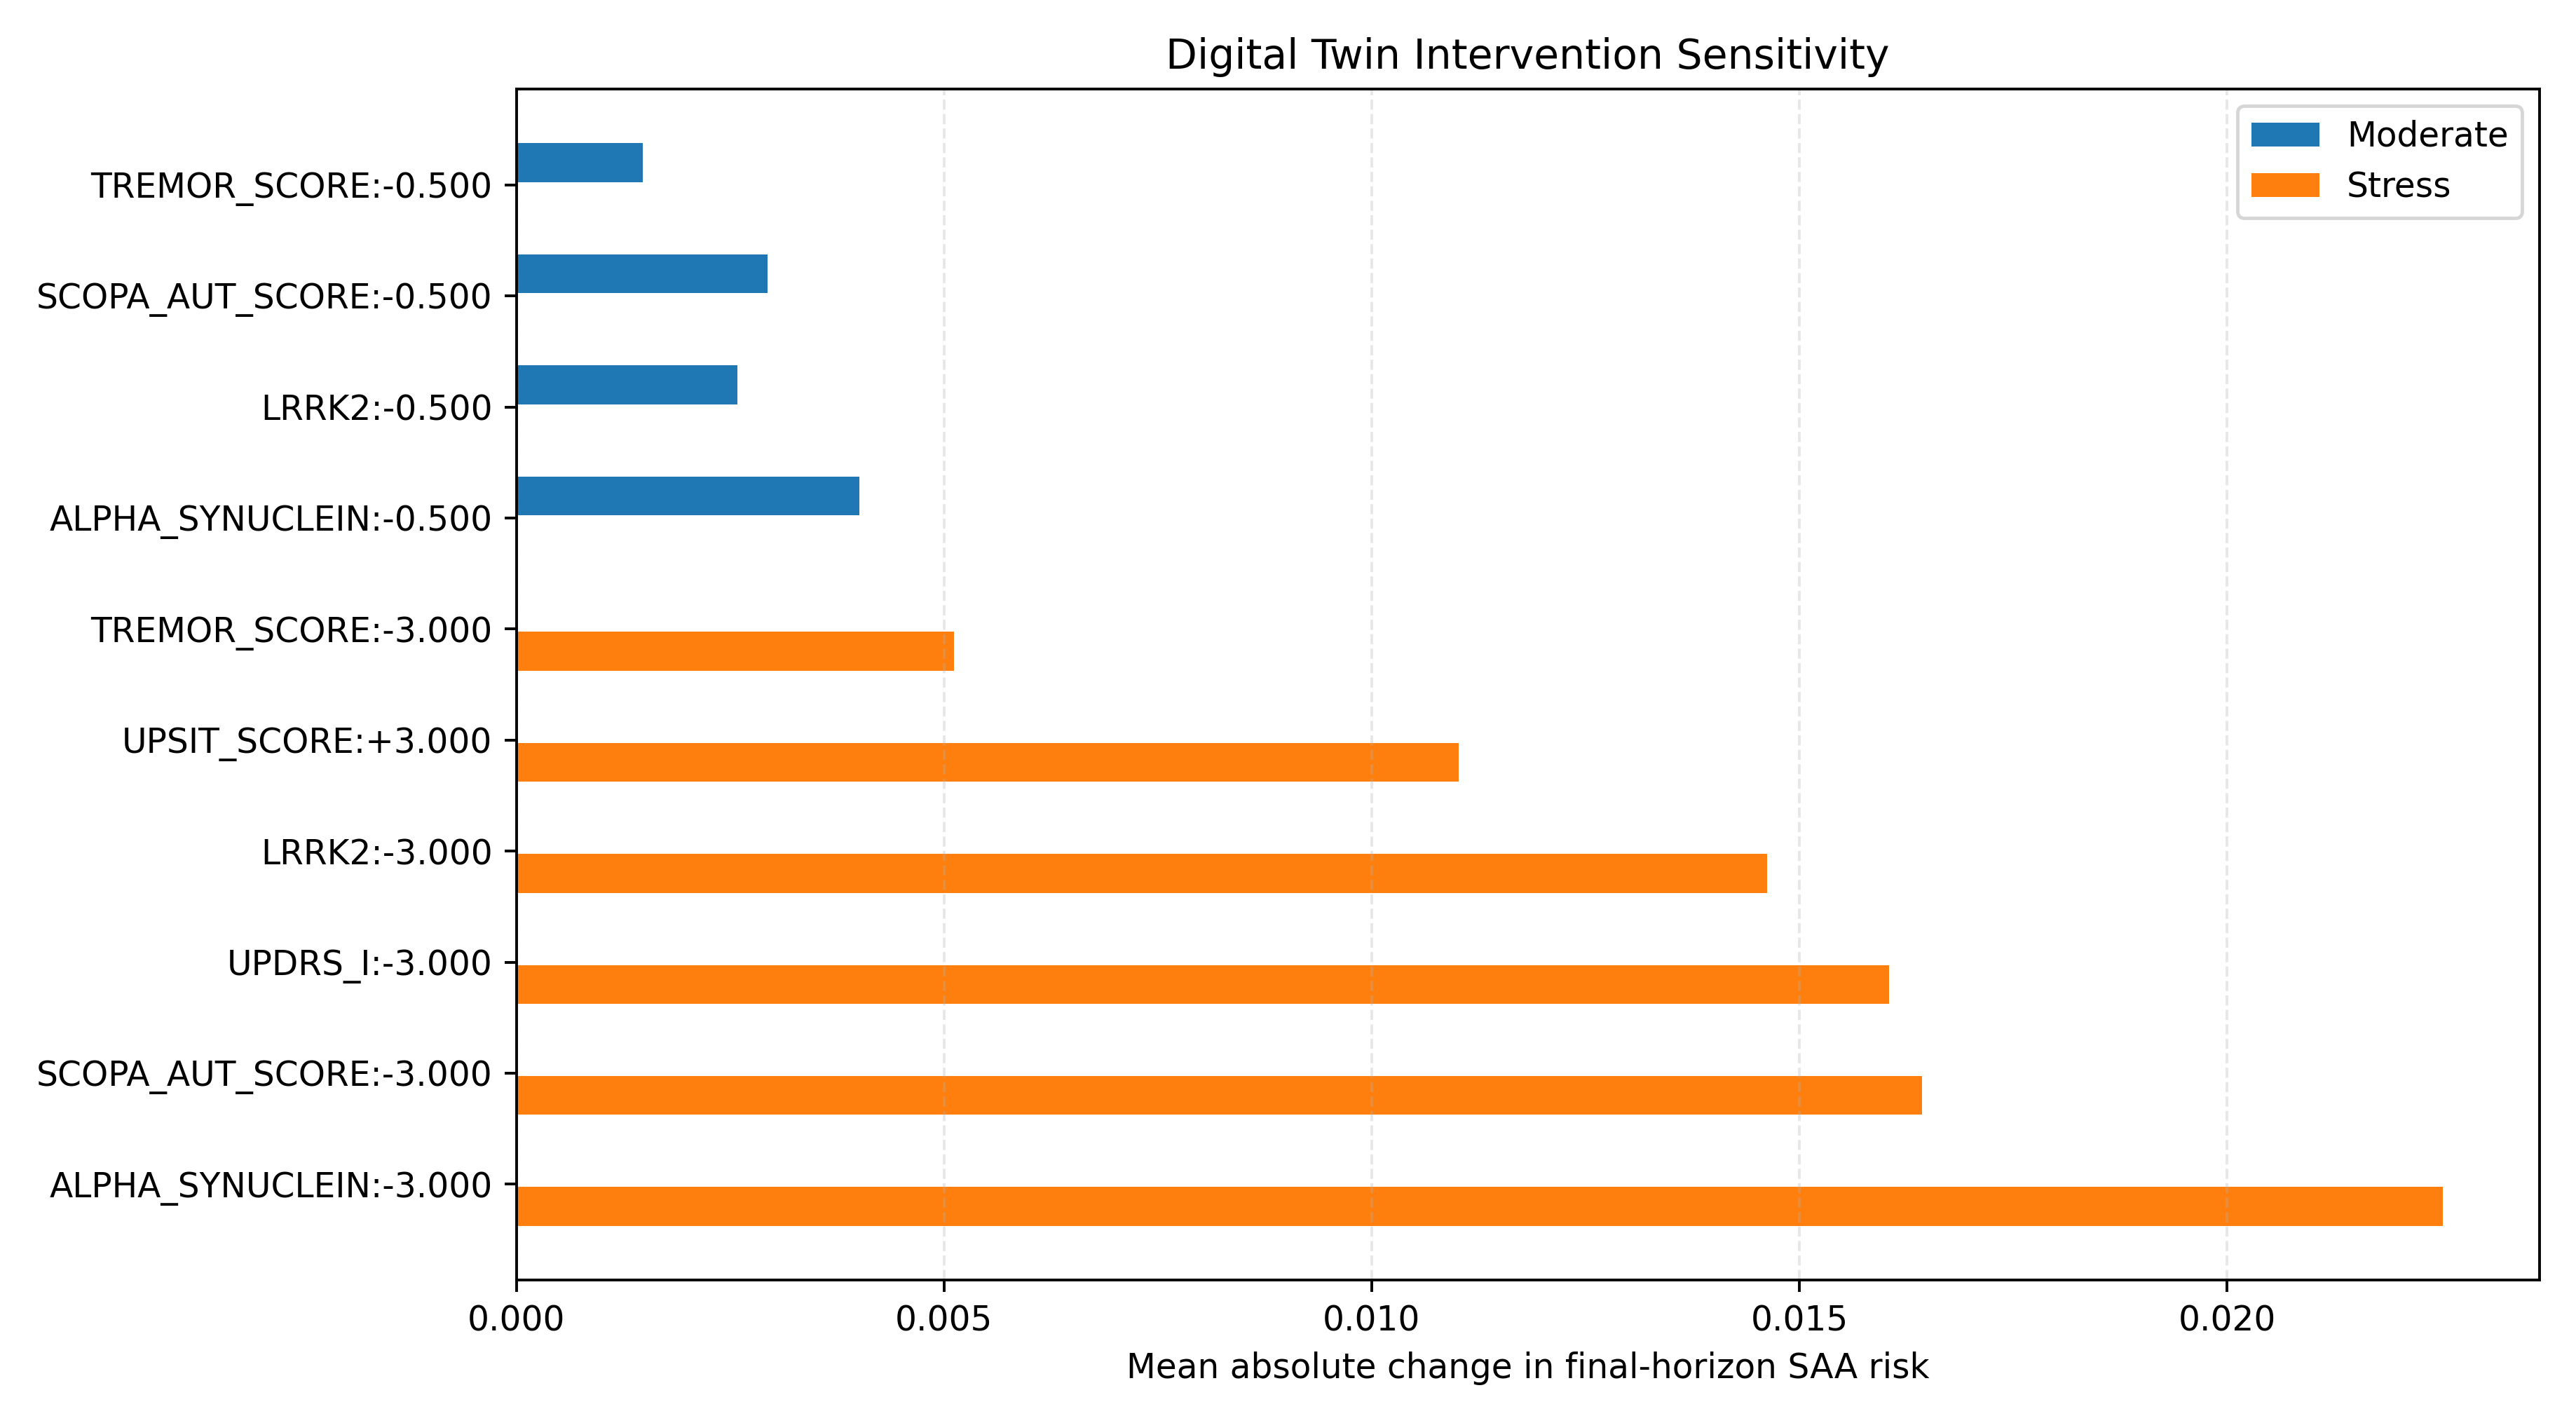
\includegraphics[width=0.92\textwidth]{../../visualizations/publication_ieee/Figure04_DigitalTwin_Sensitivity.png}
\caption{Digital twin intervention sensitivity outputs used to verify bounded counterfactual behavior.}
\label{fig:dt_sensitivity_npj}
\end{figure*}

\section{Discussion}
This work shifts FUZZY GIMAN from an innovation prototype toward a clinically credible research framework by enforcing deterministic contracts, artifact-backed reporting, and gated validation cycles. The model now supports transparent explainability and reproducible diagnostics suitable for dissertation-level defense.

The main unresolved issue is external transportability: despite internal gains, external-like disjoint pull performance was weak and survival evaluation was not estimable because of endpoint sparsity. This does not invalidate the architecture, but it does limit claim scope. The correct interpretation is ``internally rigorous, externally testable, and clinical-deployment pending.''

\section{Dissertation-Oriented Digital Twin Roadmap}
A dissertation-grade PD digital twin program can proceed through three tracks:
\begin{enumerate}
\item \textbf{Data integration track:} promote additional medication exposure, adverse events, and richer longitudinal dynamics into canonical features.
\item \textbf{Validation track:} run protocol-locked external cohorts and temporal generalization studies, with calibration and utility thresholds pre-registered.
\item \textbf{Operational twin track:} deploy scheduled update cycles with drift alarms, calibration refresh, intervention simulation, and clinician-facing audit reports.
\end{enumerate}

The current codebase already contains the core skeleton for this roadmap, including run-tagged validation and twin update artifact contracts.

\section{Limitations}
\begin{itemize}
\item External evaluation currently uses an external-like pull from the same program ecosystem, not an independent consortium cohort.
\item Positive-event sparsity in the disjoint pull limits precision and prevents survival discrimination estimation.
\item Real-time operational deployment requires additional system hardening (monitoring, governance, secure data ingress).
\end{itemize}

\section{Conclusion}
FUZZY GIMAN now has a full reproducibility and governance scaffold with publication-ready figures and artifact-backed claims. Internal performance and interpretability are competitive, but the transportability gap remains the key barrier to clinical SOTA claims. The immediate next milestone is independent external validation under the frozen protocol, followed by iterative digital twin update deployment.

\section*{Data availability}
Data used in this study are derived from PPMI resources and locally organized artifacts under the repository's data and output contracts. Run-tagged artifacts for the reported external-like analysis are available under:
\begin{itemize}
\item \texttt{outputs/external\_validation/PPMI\_20251008\_REAL\_DISJOINT/}
\item \texttt{outputs/digital\_twin\_updates/PPMI\_20251008\_REAL\_DISJOINT/}
\item \texttt{Docs/audit/EXTERNAL\_VALIDATION\_REPORT\_EV\_20260207\_PPMI\_20251008\_REAL\_DISJOINT.md}
\end{itemize}

\section*{Code availability}
Pipeline and validation scripts are available in this repository, including:
\begin{itemize}
\item \texttt{scripts/run\_external\_validation\_pipeline.py}
\item \texttt{scripts/run\_digital\_twin\_update\_cycle.py}
\item \texttt{scripts/run\_clinical\_hardening\_cycles.py}
\end{itemize}

\section*{Acknowledgements}
The authors acknowledge the PPMI program and contributing participants. Artificial intelligence tooling was used for manuscript drafting support and code-assisted reproducibility workflows.

\section*{Author contributions}
B.D. led model development, pipeline engineering, validation execution, and manuscript drafting. K.M. supervised methodology framing and technical review. Both authors approved the final manuscript.

\section*{Competing interests}
The authors declare no competing interests.

\begin{thebibliography}{99}

\bibitem{dorsey2018parkinsons}
E. R. Dorsey et al., ``The emerging evidence of the Parkinson pandemic,'' \textit{Journal of Parkinson's Disease}, vol. 8, no. s1, pp. S3--S8, 2018.

\bibitem{schapira2017nonmotor}
A. H. V. Schapira et al., ``Non-motor features of Parkinson disease,'' \textit{Nature Reviews Neuroscience}, vol. 18, no. 7, pp. 435--450, 2017.

\bibitem{fereshtehnejad2017clinical}
S.-M. Fereshtehnejad et al., ``Clinical criteria for subtyping Parkinson's disease: biomarkers and longitudinal progression,'' \textit{Brain}, vol. 140, no. 7, pp. 1959--1976, 2017.

\bibitem{poewe2017parkinson}
W. Poewe et al., ``Parkinson disease,'' \textit{Nature Reviews Disease Primers}, vol. 3, no. 1, p. 17013, 2017.

\bibitem{goetz2008movement}
C. G. Goetz et al., ``Movement Disorder Society-sponsored revision of the Unified Parkinson's Disease Rating Scale (MDS-UPDRS),'' \textit{Movement Disorders}, vol. 23, no. 15, pp. 2129--2170, 2008.

\bibitem{kuncheva2010fuzzy}
L. I. Kuncheva and F. Steimann, ``Fuzzy diagnosis,'' \textit{Artificial Intelligence in Medicine}, vol. 16, no. 2, pp. 121--128, 1999.

\bibitem{torres2006fuzzy}
A. Torres and J. J. Nieto, ``Fuzzy logic in medicine and bioinformatics,'' \textit{Journal of Biomedicine and Biotechnology}, vol. 2006, Article ID 91908, 2006.

\bibitem{zadeh1994soft}
L. A. Zadeh, ``Fuzzy logic, neural networks, and soft computing,'' \textit{Communications of the ACM}, vol. 37, no. 3, pp. 77--84, 1994.

\bibitem{zadeh1965fuzzy}
L. A. Zadeh, ``Fuzzy sets,'' \textit{Information and Control}, vol. 8, no. 3, pp. 338--353, 1965.

\bibitem{lecun2015deep}
Y. LeCun, Y. Bengio, and G. Hinton, ``Deep learning,'' \textit{Nature}, vol. 521, no. 7553, pp. 436--444, 2015.

\bibitem{goldberg1989genetic}
D. E. Goldberg, \textit{Genetic Algorithms in Search, Optimization, and Machine Learning}. Addison-Wesley, 1989.

\bibitem{marek2011ppmi}
K. Marek et al., ``The Parkinson Progression Marker Initiative (PPMI),'' \textit{Progress in Neurobiology}, vol. 95, no. 4, pp. 629--635, 2011.

\bibitem{hett2019multimodal}
K. Hett et al., ``Multimodal hippocampal subfield grading for Alzheimer's disease classification,'' \textit{Scientific Reports}, vol. 9, no. 1, p. 13845, 2019.

\bibitem{el2019predicting}
I. El-Gazzar et al., ``Predicting Parkinson's disease progression from clinical and imaging data,'' \textit{Neurobiology of Aging}, vol. 81, pp. 49--57, 2019.

\bibitem{holzinger2019causability}
A. Holzinger et al., ``Causability and explainability of artificial intelligence in medicine,'' \textit{Wiley Interdisciplinary Reviews: Data Mining and Knowledge Discovery}, vol. 9, no. 4, p. e1312, 2019.

\bibitem{wu2020comprehensive}
Z. Wu et al., ``A comprehensive survey on graph neural networks,'' \textit{IEEE Transactions on Neural Networks and Learning Systems}, vol. 32, no. 1, pp. 4--24, 2021.

\bibitem{zitnik2018modeling}
M. Žitnik et al., ``Modeling polypharmacy side effects with graph convolutional networks,'' \textit{Bioinformatics}, vol. 34, no. 13, pp. i457--i466, 2018.

\bibitem{duvenaud2015convolutional}
D. K. Duvenaud et al., ``Convolutional networks on graphs for learning molecular fingerprints,'' in \textit{Advances in Neural Information Processing Systems}, vol. 28, 2015.

\bibitem{parisot2018disease}
S. Parisot et al., ``Disease prediction using graph convolutional networks: Application to autism spectrum disorder and Alzheimer's disease,'' \textit{Medical Image Analysis}, vol. 48, pp. 117--130, 2018.

\bibitem{velickovic2018graph}
P. Veličković et al., ``Graph attention networks,'' in \textit{Proc. Int. Conf. Learning Representations}, 2018.

\bibitem{shu2021disease}
L. Shu et al., ``Disease prediction with edge-variational graph convolutional networks,'' \textit{Medical Image Analysis}, vol. 70, p. 102036, 2021.

\bibitem{pota2013fuzzy}
M. Pota et al., ``A fuzzy logic approach for ambient assisted living,'' in \textit{Proc. IEEE Int. Conf. Fuzzy Systems}, 2013, pp. 1--6.

\bibitem{kadhim2011designed}
M. A. Kadhim et al., ``Designed Fuzzy Expert System for Chronic Diseases Diagnosis,'' \textit{Babil}, vol. 1,no. 2, pp. 167--176, 2011.

\bibitem{nauck1997neuro}
D. Nauck et al., \textit{Foundations of Neuro-Fuzzy Systems}. John Wiley \& Sons, 1997.

\bibitem{guzman2005medical}
J. A. Guzmán and S. C. Mettler, ``Statistical and fuzzy inference approach to medical diagnosis,'' in \textit{Proc. Int. Fuzzy Systems Conf.}, 2005.

\bibitem{bezdek1981pattern}
J. C. Bezdek, \textit{Pattern Recognition with Fuzzy Objective Function Algorithms}. Springer Science \& Business Media, 1981.

\bibitem{jang1993anfis}
J.-S. R. Jang, ``ANFIS: Adaptive-network-based fuzzy inference system,'' \textit{IEEE Transactions on Systems, Man, and Cybernetics}, vol. 23, no. 3, pp. 665--685, 1993.

\bibitem{baltrusaitis2018multimodal}
T. Baltrusaitis et al., ``Multimodal machine learning: A survey and taxonomy,'' \textit{IEEE Transactions on Pattern Analysis and Machine Intelligence}, vol. 41, no. 2, pp. 423--443, 2019.

\bibitem{marek2001dopamine}
K. Marek et al., ``[$^{123}$I] $\beta$-CIT SPECT imaging assessment of the rate of Parkinson's disease progression,'' \textit{Neurology}, vol. 57, no. 11, pp. 2089--2094, 2001.

\bibitem{bai2018recurrent}
S. Bai et al., ``An empirical evaluation of generic convolutional and recurrent networks for sequence modeling,'' \textit{arXiv preprint arXiv:1803.01271}, 2018.

\bibitem{wen20203d}
J. Wen et al., ``Convolutional neural networks for classification of Alzheimer's disease: Overview and reproducible evaluation,'' \textit{Medical Image Analysis}, vol. 63, p. 101694, 2020.

\bibitem{choi2016doctor}
E. Choi et al., ``Doctor AI: Predicting clinical events via recurrent neural networks,'' in \textit{Machine Learning for Healthcare Conf.}, 2016, pp. 301--318.

\bibitem{nalls2019identification}
M. A. Nalls et al., ``Identification of novel risk loci, causal insights, and heritable risk for Parkinson's disease: a meta-analysis of genome-wide association studies,'' \textit{The Lancet Neurology}, vol. 18, no. 12, pp. 1091--1102, 2019.

\bibitem{ji2021dnabert}
Y. Ji et al., ``DNABERT: pre-trained bidirectional encoder representations from transformers model for DNA-language in genome,'' \textit{Bioinformatics}, vol. 37, no. 15, pp. 2112--2120, 2021.

\bibitem{avsec2021effective}
Ž. Avsec et al., ``Effective gene expression prediction from sequence by integrating long-range interactions,'' \textit{Nature Methods}, vol. 18, no. 10, pp. 1196--1203, 2021.

\bibitem{holden2018progression}
S. K. Holden et al., ``Progression of MDS-UPDRS scores over five years in de novo Parkinson disease from the Parkinson's progression markers initiative cohort,'' \textit{Movement Disorders Clinical Practice}, vol. 5, no. 1, pp. 47--53, 2018.

\bibitem{che2018recurrent}
Z. Che et al., ``Recurrent neural networks for multivariate time series with missing values,'' \textit{Scientific Reports}, vol. 8, no. 1, p. 6085, 2018.

\bibitem{katzman2018deepsurv}
J. L. Katzman et al., ``DeepSurv: personalized treatment recommender system using a Cox proportional hazards deep neural network,'' \textit{BMC Medical Research Methodology}, vol. 18, no. 1, p. 24, 2018.

\bibitem{li2018deeper}
Q. Li et al., ``Deeper insights into graph convolutional networks for semi-supervised learning,'' in \textit{Proc. AAAI Conf. Artificial Intelligence}, 2018.

\bibitem{wang2015differentiable}
G. Wang et al., ``Differentiable soft quantization: Bridging full-precision and low-bit neural networks,'' \textit{arXiv preprint arXiv:1908.05033}, 2019.

\bibitem{ying2019gnnexplainer}
R. Ying et al., ``GNNExplainer: Generating explanations for graph neural networks,'' in \textit{Advances in Neural Information Processing Systems}, vol. 32, 2019.

\bibitem{guo2017calibration}
C. Guo et al., ``On calibration of modern neural networks,'' in \textit{Proc. Int. Conf. Machine Learning}, 2017, pp. 1321--1330.

\bibitem{moons2012risk}
K. G. M. Moons et al., ``Risk prediction models: I. Development, internal validation, and assessing the incremental value of a new (bio)marker,'' \textit{Heart}, vol. 98, no. 9, pp. 683--690, 2012.

\bibitem{hamilton2017inductive}
W. L. Hamilton et al., ``Inductive representation learning on large graphs,'' in \textit{Advances in Neural Information Processing Systems}, vol. 30, 2017.

\bibitem{rudin2019stop}
C. Rudin, ``Stop explaining black box machine learning models for high stakes decisions and use interpretable models instead,'' \textit{Nature Machine Intelligence}, vol. 1, no. 5, pp. 206--215, 2019.

\bibitem{peters2017elements}
J. Peters et al., \textit{Elements of Causal Inference: Foundations and Learning Algorithms}. MIT Press, 2017.

\bibitem{kairouz2019advances}
P. Kairouz et al., ``Advances and open problems in federated learning,'' \textit{arXiv preprint arXiv:1912.04977}, 2019.

\bibitem{kazemi2020representation}
S. M. Kazemi et al., ``Representation learning for dynamic graphs: A survey,'' \textit{Journal of Machine Learning Research}, vol. 21, pp. 1--73, 2020.

\bibitem{litjens2017survey}
G. Litjens et al., ``A survey on deep learning in medical image analysis,'' \textit{Medical Image Analysis}, vol. 42, pp. 60--88, 2017.

\bibitem{eraslan2019deep}
G. Eraslan et al., ``Deep learning: new computational modelling techniques for genomics,'' \textit{Nature Reviews Genetics}, vol. 20, no. 7, pp. 389--403, 2019.

\bibitem{rajkomar2019machine}
A. Rajkomar et al., ``Machine learning in medicine,'' \textit{New England Journal of Medicine}, vol. 380, no. 14, pp. 1347--1358, 2019.

\bibitem{adeli2010fuzzy}
A. Adeli and M. Neshat, ``A fuzzy expert system for heart disease diagnosis,'' in \textit{Proc. Int. Multi-Conf. Engineers Computer Scientists}, 2010.

% Additional submission-support references
\bibitem{vickers2006decision}
A. J. Vickers and E. B. Elkin, ``Decision curve analysis: a novel method for evaluating prediction models,'' \textit{Medical Decision Making}, vol. 26, no. 6, pp. 565--574, 2006.

\bibitem{lundberg2017unified}
S. M. Lundberg and S.-I. Lee, ``A unified approach to interpreting model predictions,'' in \textit{Advances in Neural Information Processing Systems}, vol. 30, 2017.

\bibitem{van2019calibration}
B. Van Calster et al., ``Calibration: the Achilles heel of predictive analytics,'' \textit{BMC Medicine}, vol. 17, no. 1, p. 230, 2019.

\bibitem{collins2015tripod}
G. S. Collins et al., ``Transparent reporting of a multivariable prediction model for individual prognosis or diagnosis (TRIPOD): the TRIPOD statement,'' \textit{BMJ}, vol. 350, p. g7594, 2015.

\end{thebibliography}

\end{document}
